% Research note with controlled multi-seed evidence. NOT submission-ready:
% see Section "Limitations and threats to validity" and docs/next-experiments.md.
% All numbers are copied from results/experiment*/summary/tables.md.
\documentclass[11pt,a4paper]{article}
\usepackage[margin=1in]{geometry}
\usepackage{amsmath,amssymb,booktabs,graphicx,enumerate}
\usepackage[colorlinks=true,urlcolor=blue,citecolor=blue,linkcolor=blue]{hyperref}
\usepackage[numbers]{natbib}

\title{When Less Is More: Task-Relevant Coarse-Graining for\\
  Resource-Bounded Prediction in a Local Sorting System\\[0.4em]
  \large Research note --- controlled multi-seed results; not yet submission-ready}
\author{Authors to be confirmed}
\date{6 November 2026}

\begin{document}
\maketitle

\begin{abstract}
Can a deliberately compressed description of a dynamical system make its future
easier to predict for a learner with limited data and computation? We study this
question in a synthetic stochastic local-sorting system: a 64-element array that
repairs itself by unreliable neighbour exchanges. From the initial permutation and
the exchange-reliability profile we predict the mean remaining displacement after
twelve sweeps, comparing the complete 128-dimensional state, a hand-engineered
27-dimensional macroscopic summary, dimension-matched random projections and
controls, using histogram gradient-boosting regressors. Across ten independent
simulation seeds, four training budgets (250--5,000 episodes) and four capacity
presets, the macroscopic summary has lower test error than the complete state in
every seed and every cell (paired 95\% CIs exclude zero throughout). The advantage
is large when resources are scarce (43--49\% lower RMSE at 250 episodes) and
shrinks to 17\% at 5,000 episodes when each representation uses its
validation-selected capacity; both learning curves remain well above the estimated
irreducible error (0.19 vs.\ 0.33--0.40). A granularity sweep over 1--64 spatial
regions on identical episodes shows a shallow interior optimum at 8--16 regions
that disappears at small budgets and moves finer as resources grow. Feature-set
ablations attribute most of the benefit to three engineered global statistics,
especially a displacement--unreliability interaction, rather than to spatial
coarse-graining itself: three global numbers reach an error about 11\% above the best medium model,
and even a 195-feature engineered representation with a larger marginal-entropy encoding bound than
the raw state outperforms it by 26\%. Random projections do not match the engineered features at any tested
size, and a local prediction target reverses the preference for coarse
representations in every seed. We conclude that task-relevant \emph{supplied}
representations reliably improve finite-resource prediction in this system, that
the effect is a resource-dependent inductive bias rather than an information gain,
and that it is driven by the content of the summary more than by the amount of
detail discarded. A learner-free closure test then asks whether the useful
variables are a level of description of the system or merely convenient
coordinates: configurations matched on the three global summaries have futures
twelve sweeps ahead whose true conditional means agree to within 8\% of their
variance (closure index $0.918\pm0.004$), against 0.27 for a matched random
projection and 0.57 for the disorder scalar alone; re-ranking matched
configurations by microscopic detail recovers about one further point, and by
the previous macrostate a small nonzero improvement. This supports approximate conditional-mean closure for the measured
observables over the tested distribution and horizons, not full distributional
sufficiency, a general autonomous macroscopic law or Markovian dynamics. The
small nonzero history-refinement effect does not establish independence from
the past. We position these results as the first two stages of a programme on
abstraction discovery, transfer and adaptation, and propose minimal
falsification tests for the later stages. Code, raw results and figures are
released for replication.
\end{abstract}

\section{Introduction and motivation}

Borges's Funes remembers every leaf of every tree he has ever seen, and every
time he has seen it, and is for that reason almost incapable of thought: ``to
think is to forget differences, to generalize, to abstract''
\citep{borges1998}. The story is a literary conceit, not evidence, but it names
a tension that any learning system faces. A complete microscopic description of
a situation contains, by construction, at least as much information about its
future as any deterministic summary of it. For an unrestricted Bayes-optimal
predictor this is a theorem (the data-processing inequality), not a hypothesis.
For actual learners, which see finite samples and fit models of bounded
capacity in bounded time, the picture is different: some functions of the state
are much easier to learn from than others, and a summary that aligns with the
structure of the target can lower the error that a given learner reaches at a
given budget, even though the summary contains strictly less information.

This note is concerned with that gap between \emph{information available} and
\emph{information usable}. We use a small system in which it can be studied
under full control: a stochastic local-sorting process in which a disordered
64-element array repairs itself by unreliable compare-and-swap exchanges
between neighbours, inspired by (but much simpler than) the self-sorting arrays
studied as a minimal model of basal intelligence by \citet{zhang2025}. The
dynamics are known exactly, the irreducible noise in any target can be measured
by re-simulation, and the cost of every representation can be timed. The
empirical question is narrow:
\begin{quote}
\textbf{Can carefully selected macroscopic representations improve predictive
performance under finite data and computational budgets, and if so, what about
them does the work?}
\end{quote}
We ask it in four forms. Does a hand-engineered macroscopic representation
reliably beat the complete microscopic state across independent seeds,
training budgets and learner capacities, including when the raw-state learner
is free to choose its capacity on validation data (Experiment~1)? How much
spatial detail can be removed before performance degrades, and is there an
optimal intermediate scale (Experiment~2)? Is any benefit attributable to
coarse-graining as such, to the particular engineered statistics, or merely to
dimensionality (ablations within Experiment~2)? And, independently of any
learner, do configurations with similar summaries have similar conditional-mean
futures for the measured observables (Experiment~2b)?

The question is one component of a broader interest, which we state here so
that the limits of the present contribution are clear. The working hypothesis
behind this programme is that an important mechanism of intelligent behaviour,
in natural and artificial systems alike, is the capacity to discover, construct
and reuse task-relevant abstractions: to identify in a new situation which
distinctions matter for the current objective, to preserve the relationships
among them while discarding the rest, and to revise that choice when the
objective or the situation changes. Three capabilities follow:
\emph{abstraction discovery}, \emph{abstraction transfer} to structurally
related situations, and \emph{abstraction adaptation} when a previously
successful representation stops being adequate. We return to this framing, to
its relation to existing theories, and to how it might be tested, in
Sections~\ref{sec:discussion} and~\ref{sec:future}. \textbf{None of the three
capabilities is tested here.} The macroscopic features in our experiments are
hand-engineered with knowledge of the sorting objective; the experiments test
whether \emph{supplied} abstractions improve resource-bounded prediction, which
is a prerequisite for the programme rather than a demonstration of it.

A further hypothesis, also stated here and also untested, concerns where
useful abstractions come from. The macroscopic variables that make a
many-body system predictable are often not inventions of the observer but
reflections of its collective organization: pressure and velocity fields exist
because molecular collisions produce them, and they predict the fluid because
the fluid's dynamics approximately close over them. We conjecture that
\textbf{some emergent macroscopic properties are particularly useful targets
for abstraction because they capture stable, predictive relationships among
microscopic variables}, and that a system able to find such levels of
description would have an advantage in prediction. Two cautions apply.
\emph{Emergence} is a property of the system's organization and dynamics;
\emph{abstraction} is a property of how an observer or model represents it. An
emergent regularity can exist unrecognized; an abstraction can be useful
without corresponding to any recognized emergent law; and a compressed
representation need not reveal emergent structure at all. The two are related
by a correspondence that must be established case by case. Experiments~1
and~2 do not establish it: our features were chosen with knowledge of the
sorting objective, for which disorder and displacement are natural, almost
obvious, quantities. Experiment~2b tests the weakest useful form of the
correspondence, approximate predictive closure, directly and without a
learner.

Two further distinctions are used throughout. \emph{Compression} reduces the
amount of information; \emph{abstraction} aims to preserve the structure that
makes information useful for a task. A representation can be compact without being
useful (our random projections) and useful without being compact (our
195-feature engineered representation). Likewise, \emph{having} information,
\emph{representing} it usefully, \emph{predicting} efficiently from it, and
\emph{generalizing or transferring} what was learned are related but distinct
achievements; the experiments below bear on the first three only within one
simulator.

\section{Related work}

\paragraph{Information bottleneck and predictive compression.}
\citet{tishby2000} define the representation $Z$ of an input $X$ that is most
informative about a target $Y$ at a given compression level by minimizing
$I(X;Z)-\beta I(Z;Y)$; \citet{alemi2017} give a variational neural
implementation. The data-processing inequality guarantees $I(Z;Y)\le I(X;Y)$
for any $Z=f(X)$, so a deterministic summary can never contain \emph{more}
information about the target. Any practical advantage must therefore come from
finite data, bounded capacity, computational cost or inductive bias, which is
exactly what our experiments vary. Three notions that are often conflated must
be kept apart: information-theoretic compression (a property of
distributions), feature dimensionality (a property of a coding), and
representational complexity as seen by a learner (a property of the coding
\emph{and} the learner). Our random projections have low dimensionality and
high marginal entropy; our 64-bin engineered representation has high
dimensionality, a larger entropy bound than the raw state, and the lowest
learner-facing complexity of the three. Our macroscopic features are not
optimized under any bottleneck objective and we estimate no mutual
information.

\paragraph{Sufficient statistics and predictive representations.}
Computational mechanics \citep{shalizi2001,crutchfield2012} characterizes the
causal states of a process: histories are grouped into one state when they
imply the same distribution over futures, which yields the minimal statistic
of the past that is sufficient for the future. Optimal causal inference
\citep{still2010} approximates causal states under resource limits; predictive
information \citep{bialek2001} measures how much of the future the past
determines; predictive state representations \citep{littman2002} replace
latent state by a set of predictions about future observations.
\citet{shalizimoore2003} apply the same idea to physical macrostates: starting
from a set of observables, refine the partition of phase space until the
resulting states predict their own future, that is, until the coarse-grained
process is Markov. These are properties of a process, defined without
reference to a learner. We measure what a particular finite-sample learner
attains from candidate summaries, which the information ordering of
Section~\ref{sec:estimand} relates to, but does not identify with,
sufficiency. The computational-mechanics construction is, however, exactly the
kind of criterion by which an \emph{autonomously discovered} abstraction could
be judged, and we return to it in Sections~\ref{sec:emergent}
and~\ref{sec:future}.

\paragraph{Coarse-graining, effective theories and renormalization.}
Kadanoff's block spins \citep{kadanoff1966} and the renormalization group
explain why a few macroscopic variables can describe collective behaviour near
criticality, and \citet{kochjanusz2018} show that a mutual-information
criterion can recover such coarse-grainings from data. Fluid mechanics is the
everyday example: the Navier--Stokes equations relate density, pressure and
velocity fields without representing molecules, and are predictive wherever
the continuum description holds. Two caveats from that tradition apply to us.
An effective description is adequate within a regime, not universally; and a
compact governing law need not make prediction cheap (chaos; computational
irreducibility \citep{wolfram1985}). Our spatial-bin sweep is a crude,
data-driven analogue of coarse-graining with no claim about fixed points or
universality.

\paragraph{State abstraction in sequential decision making.}
The reinforcement-learning literature has formal treatments of much of what
``task-relevant abstraction'' means. \citet{li2006} unify state-aggregation
schemes by what they preserve (model, $Q$-values, optimal actions);
bisimulation metrics \citep{ferns2004} quantify how far two states may be
merged without changing achievable value; \citet{abel2020} proposes desiderata
for abstractions (near-optimal behaviour, efficient learnability and
construction, reduced planning or learning cost) and proves trade-offs among
them. \citet{ho2022} show experimentally that people construct simplified task
representations when planning, attending to a subset of objects that depends on
the task. Our setting is supervised prediction rather than control, but the
questions overlap: what must a representation preserve for the task, and what
does it cost to build and to use.

\paragraph{Statistical learning and inductive bias.}
Gradient-boosted trees are strong learners on tabular data of this size
\citep{grinsztajn2022,ke2017} and are known to be sensitive to how features
are expressed, learning axis-aligned, irregular functions well and smooth
rotated ones poorly \citep{grinsztajn2022}. The macro--raw gap we report is,
in part, a statement about this inductive bias meeting a particular coding of
the state; we use random projections \citep{bingham2001} as a control for
dimensionality and discuss locality-aware architectures as the missing
competitor.

\paragraph{Emergence and collective dynamics.}
\citet{zhang2025} study sorting algorithms as a model of morphogenesis and
report collective competencies in self-sorting arrays; Levin
\citep{levin2019,levin2022} frames cognition as scale-free, with collectives of
cells solving problems in spaces their components do not represent. In
physics, \citet{cavagna2010} showed that starling flocks exhibit scale-free
velocity correlations, so that the useful predictive variables of the flock
live at a level of description different from the individual bird. Four
notions should be kept distinct here: \emph{emergence} (macroscopic
regularities produced by local interactions), \emph{self-organization} (the
process by which they arise without central control), \emph{adaptation}
(change in response to feedback) and \emph{intelligence} (in our working
sense, the efficient discovery and reuse of task-relevant abstractions). Our
simulator borrows the first two in their simplest form (local rules, global
order) but not the biology; the emergence of a macroscopic pattern does not
make it easy to predict, nor does it imply intelligence.

\paragraph{Predictive autonomy of coarse-grained dynamics.}
When does a macroscopic description predict its own future? For a Markov
chain, a partition of the state space is \emph{lumpable} when the
coarse-grained process is itself Markov \citep{kemeny1976}; informational
closure \citep{pfante2014} generalizes the idea to $I(Z_{t+1};X_t\mid Z_t)=0$,
the condition that the microstate adds nothing to the macrostate for
predicting the next macrostate; \citet{seth2010} proposes Granger-causal
measures of the autonomy of a process from its substrate.
\citet{israeli2006} showed constructively that many one-dimensional cellular
automata, including computationally irreducible ones, admit coarse-grainings
whose dynamics are closed and often simpler than the microscopic rule, so that
a system can be unpredictable in detail and predictable at some level of
description. These are the formal tools for the question of
Section~\ref{sec:emergent}, whether our macroscopic variables approximately
close over themselves; Experiment~2b tests agreement in conditional means, a necessary but
insufficient part of full distributional closure.

\paragraph{Causal emergence.}
\citet{hoel2013} and \citet{hoel2017} argue that, under an interventionist
account of causation and a maximum-entropy distribution over interventions, a
coarse-grained causal model can carry more \emph{effective information} than
the microscopic model from which it is built; \citet{rosas2020} give an
alternative, observational information-theoretic formalization. Both have been
criticized: \citet{dewhurst2021} argues that effective-information causal
emergence is at most epistemic, and \citet{eberhardt2022} show that the
macro-level interventions are ambiguous and that abstraction and
marginalization fail to commute, tracing the apparent gain to averaging steps
and to a distribution that is not the system's own. We take no position on
this debate. What matters for us is the distinction it makes vivid:
\emph{observational predictive sufficiency} (a macrostate predicts the future
macrostate as well as the microstate does) is a weaker and better-defined
property than \emph{causal emergence}, and Experiment~2b measures only agreement in conditional means, which is weaker
still than full observational predictive sufficiency.

\paragraph{Representation transfer and analogy.}
Gentner's structure-mapping theory \citep{gentner1983} holds that analogy is a
mapping of relations, not of object attributes, and that systems of
higher-order relations are preferentially carried across: a chess player
learning a new board game transfers notions like territory and sacrifice, not
the shapes of the pieces. Transfer learning \citep{pan2010} studies when
knowledge from a source domain reduces the data needed in a target domain, and
when it hurts (negative transfer). \citet{chollet2019} defines intelligence as
skill-acquisition efficiency over a scope of tasks, controlling for prior
knowledge and experience, and argues that benchmarks must account for priors.
These frameworks motivate the later stages of our programme
(Section~\ref{sec:future}) and are not tested here; in particular, success
across random seeds of one simulator is not transfer.

\paragraph{Positioning.}
The working hypothesis in the Introduction is a synthesis, not a new theory.
Its emphasis on efficiency given priors is Chollet's; its emphasis on
relational structure is Gentner's; its criteria for a good abstraction
(near-sufficiency, cheap to build, cheap to use) are Abel's and Li et al.'s;
its information-theoretic core is the bottleneck; and its emergence component
is the macrostate construction of Shalizi and Moore and the coarse-graining
programme of Israeli and Goldenfeld, applied to a learner rather than to a
physicist. What this note adds is
empirical and narrow: a fully controlled system with measurable noise floor in
which the contributions of content, resolution, dimensionality, capacity, data
and compute to the usefulness of a supplied abstraction can be separated, and
in which the task dependence of the answer can be shown directly.

\section{Experimental system}

The simulator is a simplified stochastic odd--even transposition process,
inspired by but not a reproduction of \citet{zhang2025}. An array holds a
permutation of $0,\ldots,63$; episodes begin sorted and are disturbed by
shuffling one contiguous block (probability 0.75) or two (0.25), with block
widths 5--32. Every one of the 63 adjacent edges has an exchange reliability of
0.90 except a fault interval of width 5--20 with a single reliability drawn from
$[0.15,0.65)$. A sweep applies compare-and-swap to all even-indexed edges and
then all odd-indexed edges; an inverted pair is swapped with its edge's
reliability probability. A \emph{shifted} test distribution uses fault widths
5--30 and reliabilities in $[0.05,0.30)$.

The global target is
\begin{equation}
  Y_H=\frac{1}{64}\sum_{i=0}^{63}\lvert a_H[i]-i\rvert,\qquad H=12,
\end{equation}
in positions per element (mean $\approx 0.9$, SD 1.18 on the test
distribution). The local control target is the value at position 32 after one
sweep. Both are random given the initial state. We estimate the irreducible RMSE
by re-simulating each test episode 32 times: $0.192\pm0.003$ for the global
target and $3.01\pm0.10$ for the local target (mean $\pm$ SD over seeds).

\section{Representations and prediction tasks}

All representations are deterministic functions of the initial state; none uses
the future. The \textbf{full state} is the 64 normalized values and 64
reliabilities (128 features). The \textbf{macroscopic} representation has three
\emph{global} statistics---mean normalized displacement, fraction of adjacent
descents, and the mean over edges of displacement $\times$ $(1-\text{reliability})$---plus
three \emph{regional} statistics per spatial bin (mean displacement, descent
fraction, mean unreliability), the 64 positions being split into $B$ contiguous
bins. The baseline uses $B=8$ (27 features). Two edge-assignment rules exist:
the original \emph{interior} rule counts only edges fully inside a bin and is
defined for $B\le 32$; a \emph{left} rule assigns every edge to the bin of its
left position and extends to $B=64$. Both give indistinguishable results where
they overlap. At every resolution, including 64 bins, element identities and
the sign of each displacement are discarded; the 64-bin representation is
therefore not the raw state. \textbf{Initial disorder} is the first global
statistic alone. The \textbf{random projection} multiplies the standardized full
state (standardizer fitted on the training subset only) by a fixed Gaussian
matrix with $3+3B$ columns. \textbf{Full + macro} concatenates the full state
and the macroscopic features as a diagnostic.

We also report representation-size proxies: feature count, a marginal-entropy
encoding bound (each feature discretized into $\le 255$ quantile bins, as the
learner does internally; entropies summed, which upper-bounds the joint entropy
of the discretized representation), effective rank, and mean absolute
inter-feature correlation. These are bounds and redundancy measures, not
mutual-information estimates.

The cost of \emph{constructing} the macroscopic features is not represented in
any of our measurements: they were designed by hand using knowledge of the
sorted goal configuration and of the fault mechanism. A representation that is
cheap to apply (ours costs 2.6\,ms per 5,000 episodes) may be expensive to
discover, and the discovery cost is the quantity the later stages of the
programme are about.

\section{Experimental methodology}

\subsection{Estimand}\label{sec:estimand}
For target $Y$ and initial state $X_0$, any deterministic summary $Z=f(X_0)$
satisfies $\mathcal{R}^*(X_0)\le\mathcal{R}^*(Z)$ for the Bayes risk under
squared error. Our experiments estimate the \emph{attained} risk
$\mathcal{R}(\hat f;\mathcal{D}_n,\mathcal{A})$ of a learning algorithm
$\mathcal{A}$ trained on $n$ episodes, and the comparison of interest is between
representations at matched $n$, matched estimator settings, matched realised
model size, and (separately) matched wall-clock cost.

\subsection{Learner and capacity presets}
All conditions use \texttt{HistGradientBoostingRegressor} \citep{pedregosa2011}
with learning rate 0.075, minimum leaf size 12, $\ell_2$ regularization 2.0 and
no early stopping. Capacity presets vary only the number of trees and maximum
leaves per tree: small ($50\times4$), medium ($100\times9$, the baseline),
large ($300\times31$) and xlarge ($1{,}000\times63$). Realised ensemble sizes
(900 leaves at medium, 9,300 at large, 63,000 at xlarge) are identical across
representations at a preset, so a within-preset comparison is matched in
parameter count.

\subsection{Data, splits and randomness}
Every random stream is \texttt{numpy.random.default\_rng(seed + offset)} with
documented offsets. Per seed we simulate a 5,000-episode training pool, 1,000
validation episodes, 2,000 in-distribution and 2,000 shifted test episodes.
Training budgets are nested prefixes of the pool, so all representations and
capacities see exactly the same episodes at a budget. Seeds are
$1000,2000,\ldots,10000$. Hyperparameter (capacity) selection uses validation
RMSE only; test splits are never used for selection. With the baseline seed the
pipeline reproduces the single-seed baseline exactly at the 5,000 budget.

\subsection{Statistics and costs}
We report means, SDs and 95\% $t$-intervals across seeds, paired across-seed
differences with $t$ and Wilcoxon signed-rank tests, and the number of seeds in
which one representation beats another. Wall-clock feature extraction (median
of five repeats), fitting and inference on 2,000 episodes are measured on one
machine (Apple Silicon, 10 cores, default OpenMP threading); they order
configurations but are not portable benchmarks.

\section{Experiment 1: robustness and model capacity}

\paragraph{Design.}
10 seeds $\times$ budgets $\{250,750,2000,5000\}$ $\times$ presets
$\{\text{small},\text{medium},\text{large}\}$ $\times$ 5 representations
$\times$ 2 tasks, plus xlarge at 5,000 on the global task (its cost,
$\sim$20\,s per fit, made the full grid unreasonable). In addition to
fixed-preset comparisons we report a \emph{validation-selected} comparison in
which each representation uses, per seed and budget, the preset with the lowest
validation RMSE. This lets a raw-state model choose more capacity if that helps
it.

\paragraph{Falsification criteria.}
The baseline interpretation fails if the macro--full difference is not
consistently negative across seeds, if it is eliminated by capacity selection,
or if the random projection matches the macro representation (which would
attribute the effect to dimensionality rather than content).

\section{Experiment 2: spatial coarse-graining}

\paragraph{Design.}
On the same episodes within each seed: macro, regional-only and
random-projection representations at $B\in\{1,2,4,8,16,32,64\}$, plus
global-only (3 features) and raw (128) references, at the medium preset for
every budget; small and large presets at 250 and 5,000 for a granularity
$\times$ capacity grid; the local control for macro at every $B$; size proxies
on the training pool; permutation importance on the validation split for the
8-bin model at 5,000.

\paragraph{Falsification criteria.}
The coarse-graining interpretation fails if error decreases monotonically with
$B$ (detail always helps), or if global-only performance equals the best macro
performance (regional detail is irrelevant). A regional-only ablation isolates
the effect of resolution from the global statistics.

\section{Experiment 2b: emergent predictive structure (closure test)}\label{sec:exp2b-design}

\paragraph{Design.}
Per seed, 10,000 configurations from the episode distribution advanced by two
sweeps (so a one-sweep history exists), each simulated forward 16 times,
recording the three global summaries after every sweep to $\tau=12$. For a
candidate abstraction $\phi$, each configuration is matched to its $k=10$
nearest \emph{distinct} configurations in standardized $\phi$-space; with
$\mu_i$ the realisation mean of the future, the excess variance is the pair
mean of $(\mu_i-\mu_j)^2/2$ corrected for realisation noise, and the closure
index is $1-\text{excess}/V_{\text{total}}$, where $V_{\text{total}}$ is the
noise-corrected variance of conditional means across configurations. A closure
of 1 means no residual disagreement in conditional means in this diagnostic;
it does not imply identical future distributions. Candidates: initial disorder (1), global (3), macro at 1--32 bins,
regional-8, random projections of 3/6/27/99 dimensions, and the raw state. The
estimator is biased downward for high-dimensional $\phi$, whose neighbours are
farther apart, so it is also computed at 2,500 and 5,000 configurations as a
convergence check and comparisons are made at matched size. Two-stage
refinements ask whether more information adds to the macrostate without the
dimensional confound: the 50 nearest in $\phi$ are re-ranked by raw-state
distance (\texttt{+raw}), by the previous sweep's global summaries
(\texttt{+history}), by the present global summaries (\texttt{+global}, the
control for history) or at random (\texttt{+random}, the control for
re-ranking).

\paragraph{Falsification criteria.}
The emergence reading fails if the global or macro-8 closure is not clearly
above that of a random projection of matched size, or not clearly above the
disorder scalar at the full horizon; it is qualified if raw re-ranking
recovers a large part of the residual (microscopic detail matters) or if
history re-ranking beats present-global re-ranking (evidence of history
dependence in these conditional means, rather than a complete Markov test).

\section{Results}

\subsection{Experiment 1}

\begin{figure}[t]
  \centering
  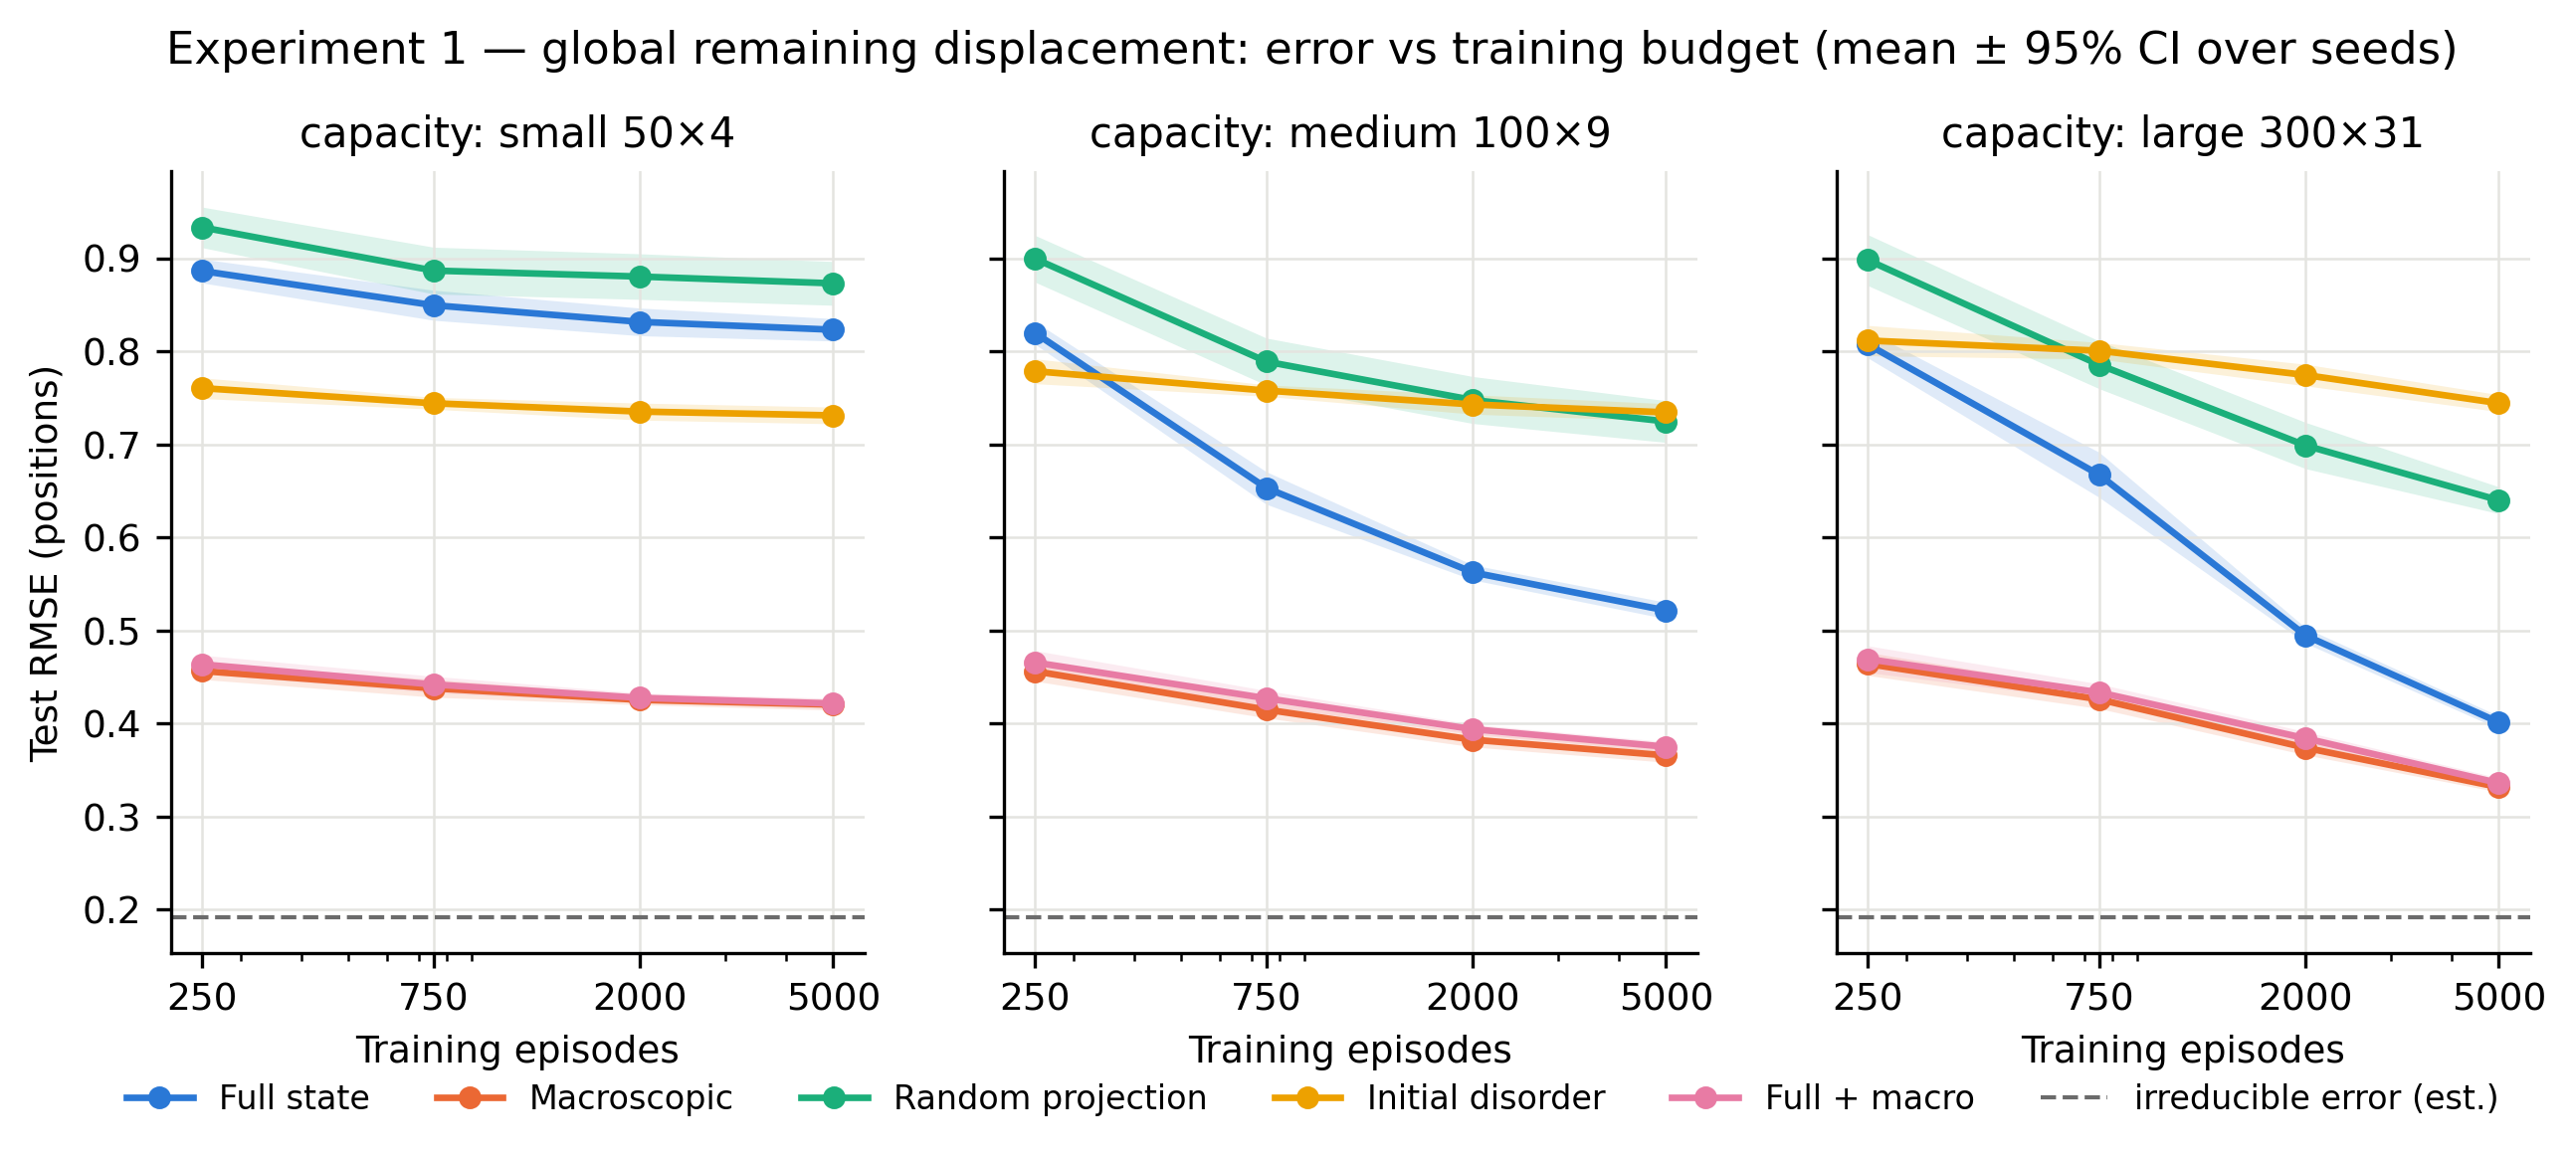
\includegraphics[width=\linewidth]{figures/exp1_learning_curves.png}
  \caption{Global-task test RMSE vs.\ training budget for each capacity preset
  (mean $\pm$ 95\% CI over 10 seeds). Dashed line: estimated irreducible error.}
  \label{fig:curves}
\end{figure}

\begin{table}[t]
\centering
\caption{Global-task test RMSE (positions; mean $\pm$ SD over 10 seeds).}
\label{tab:exp1}
\small
\begin{tabular}{llrrrrr}
\toprule
Capacity & $n$ & Full state & Macroscopic & Random proj. & Init.\ disorder & Full+macro\\
\midrule
medium & 250   & $0.820\pm0.017$ & $0.456\pm0.015$ & $0.900\pm0.035$ & $0.779\pm0.019$ & $0.466\pm0.018$\\
medium & 5,000 & $0.521\pm0.012$ & $0.366\pm0.010$ & $0.725\pm0.031$ & $0.734\pm0.013$ & $0.375\pm0.008$\\
large  & 250   & $0.807\pm0.020$ & $0.464\pm0.017$ & $0.898\pm0.038$ & $0.812\pm0.023$ & $0.469\pm0.020$\\
large  & 5,000 & $0.401\pm0.010$ & $0.332\pm0.007$ & $0.640\pm0.020$ & $0.744\pm0.013$ & $0.336\pm0.008$\\
xlarge & 5,000 & $0.420\pm0.010$ & $0.341\pm0.010$ & $0.644\pm0.021$ & $0.745\pm0.013$ & $0.349\pm0.008$\\
val.-selected & 250   & $0.807\pm0.020$ & $0.455\pm0.014$ & $0.897\pm0.036$ & $0.760\pm0.016$ & $0.461\pm0.016$\\
val.-selected & 5,000 & $0.401\pm0.010$ & $0.332\pm0.007$ & $0.641\pm0.020$ & $0.731\pm0.013$ & $0.336\pm0.008$\\
\bottomrule
\end{tabular}
\end{table}

\begin{table}[t]
\centering
\caption{Paired difference Macroscopic $-$ Full state in test RMSE (10 seeds;
macro lower in 10/10 seeds in every row; paired $t$ $p<10^{-6}$, Wilcoxon
$p=0.002$).}
\label{tab:paired}
\begin{tabular}{lrlr}
\toprule
Setting & Mean diff & 95\% CI & Relative\\
\midrule
small, 250 & $-0.430$ & $[-0.441,-0.419]$ & $-48.5\%$\\
medium, 5,000 & $-0.156$ & $[-0.170,-0.142]$ & $-29.9\%$\\
large, 5,000 & $-0.070$ & $[-0.079,-0.060]$ & $-17.4\%$\\
xlarge, 5,000 & $-0.079$ & $[-0.091,-0.068]$ & $-18.8\%$\\
validation-selected, 250 & $-0.353$ & $[-0.369,-0.337]$ & $-43.7\%$\\
validation-selected, 5,000 & $-0.070$ & $[-0.079,-0.060]$ & $-17.4\%$\\
\bottomrule
\end{tabular}
\end{table}

The macro representation beats the full state in every one of the 130 seed
$\times$ budget $\times$ capacity cells (Tables~\ref{tab:exp1}
and~\ref{tab:paired}, Figure~\ref{fig:curves}). The advantage is 43--49\% at
250 episodes and declines with both budget and capacity to 17\% at 5,000
episodes under validation-selected capacity (large for both representations).
The raw-state curve is still falling steeply at 5,000 episodes ($0.494\to0.401$
from 2,000 to 5,000 at large) while the macro curve is flattening
($0.374\to0.332$); both remain far above the 0.192 floor. The xlarge preset is
worse than large for every representation, consistent with over-fitting under a
fixed learning rate without early stopping; validation selection never chooses
it for the macro or full representations.

Controls: the random projection has higher mean error than macro and full state
at every tested budget and capacity (macro $-$ random $=-0.30$ to $-0.48$, 46--52\% relative, 10/10
seeds), worse than the single disorder scalar at the smallest budget, but not in
every setting. Full + macro
is marginally \emph{worse} than macro alone in every cell (by 0.001--0.012;
macro lower in 8--10 of 10 seeds). On the shifted split the macro advantage is
larger (large/5,000: $0.336\pm0.014$ vs.\ $0.481\pm0.021$, paired $-0.145$
$[-0.158,-0.132]$).

\begin{figure}[t]
  \centering
  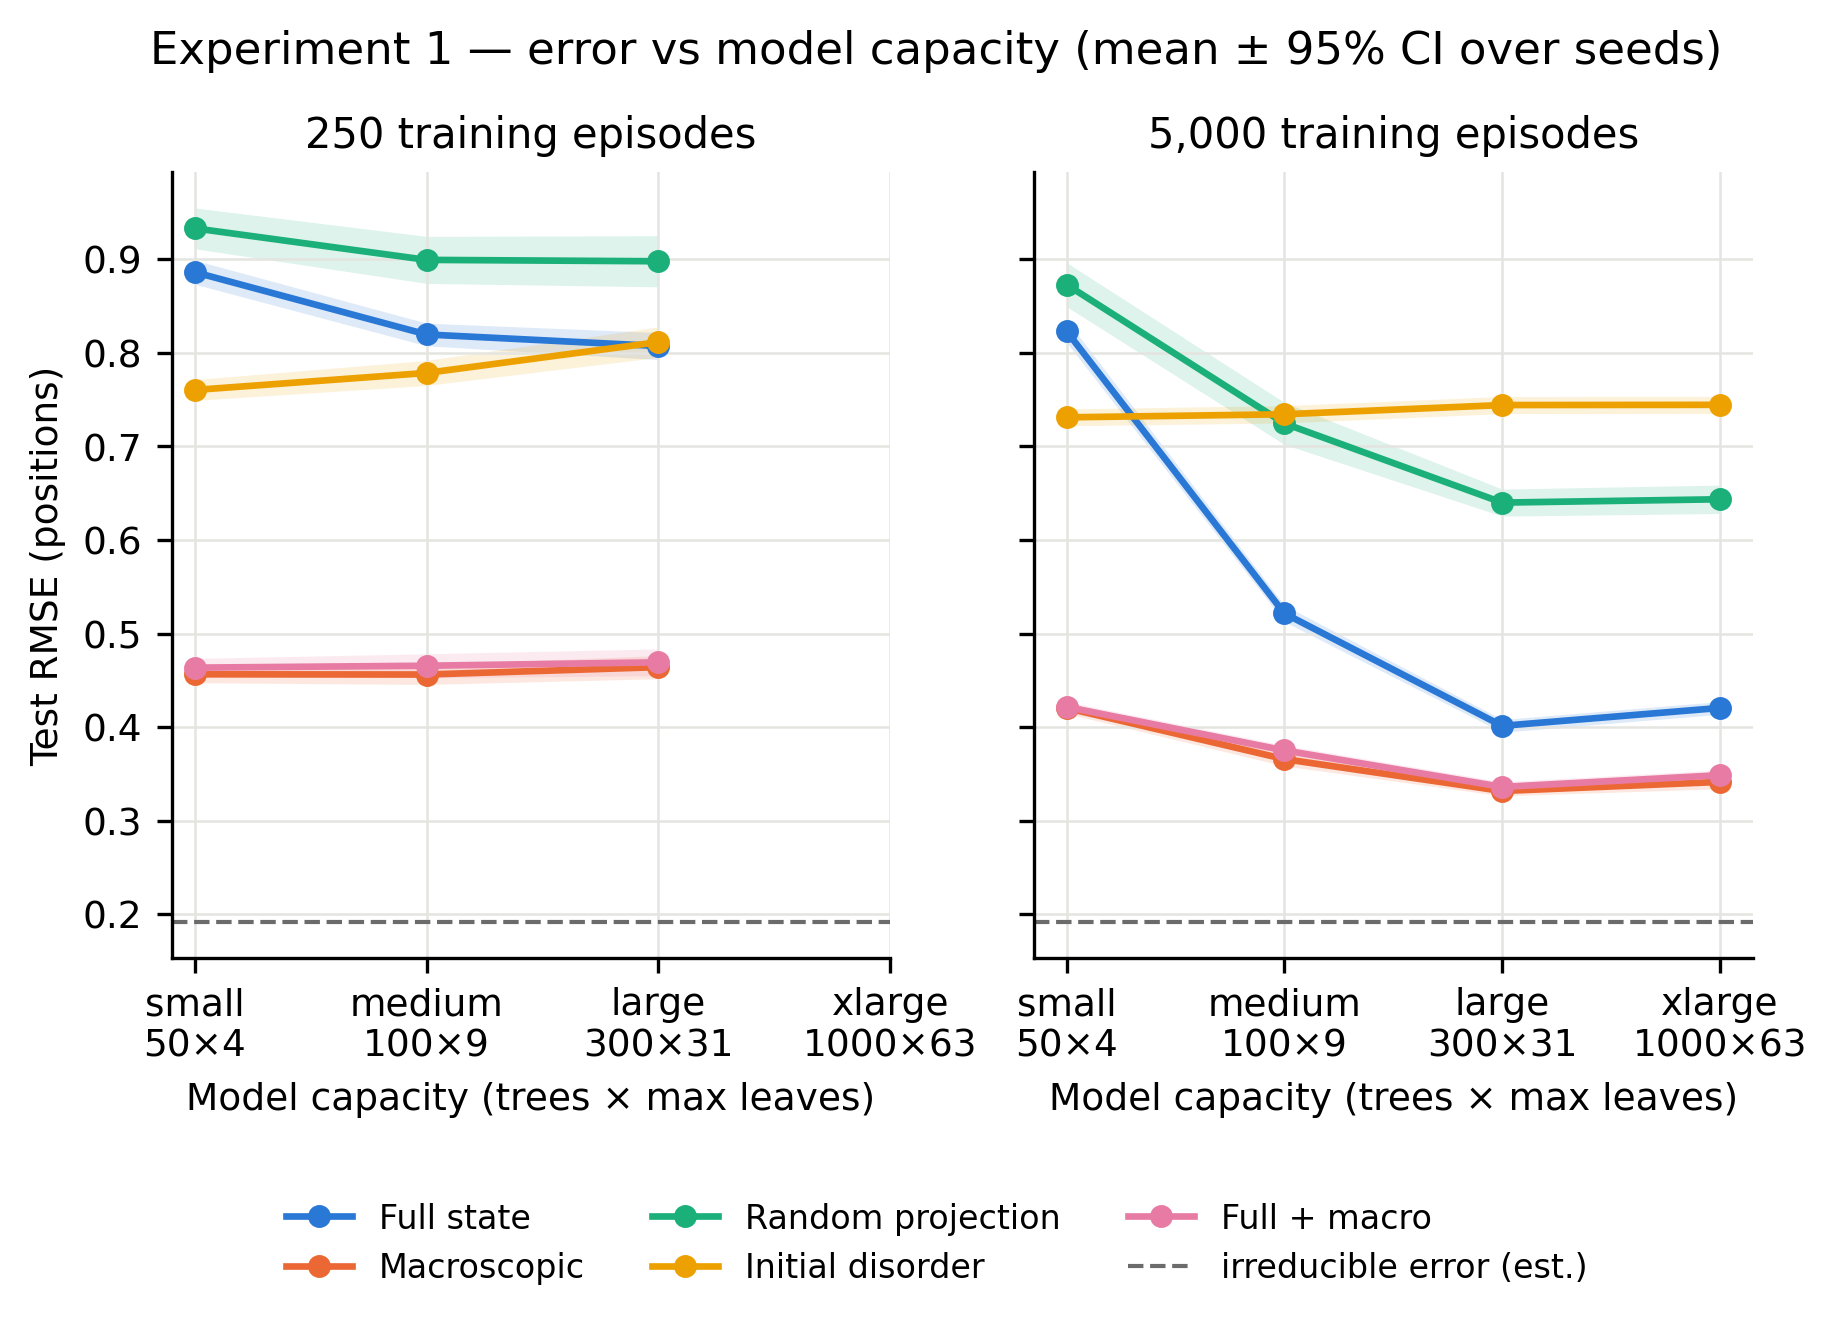
\includegraphics[width=0.8\linewidth]{figures/exp1_capacity.png}
  \caption{Test RMSE vs.\ capacity preset at 250 and 5,000 training episodes.}
  \label{fig:capacity}
\end{figure}

\begin{figure}[t]
  \centering
  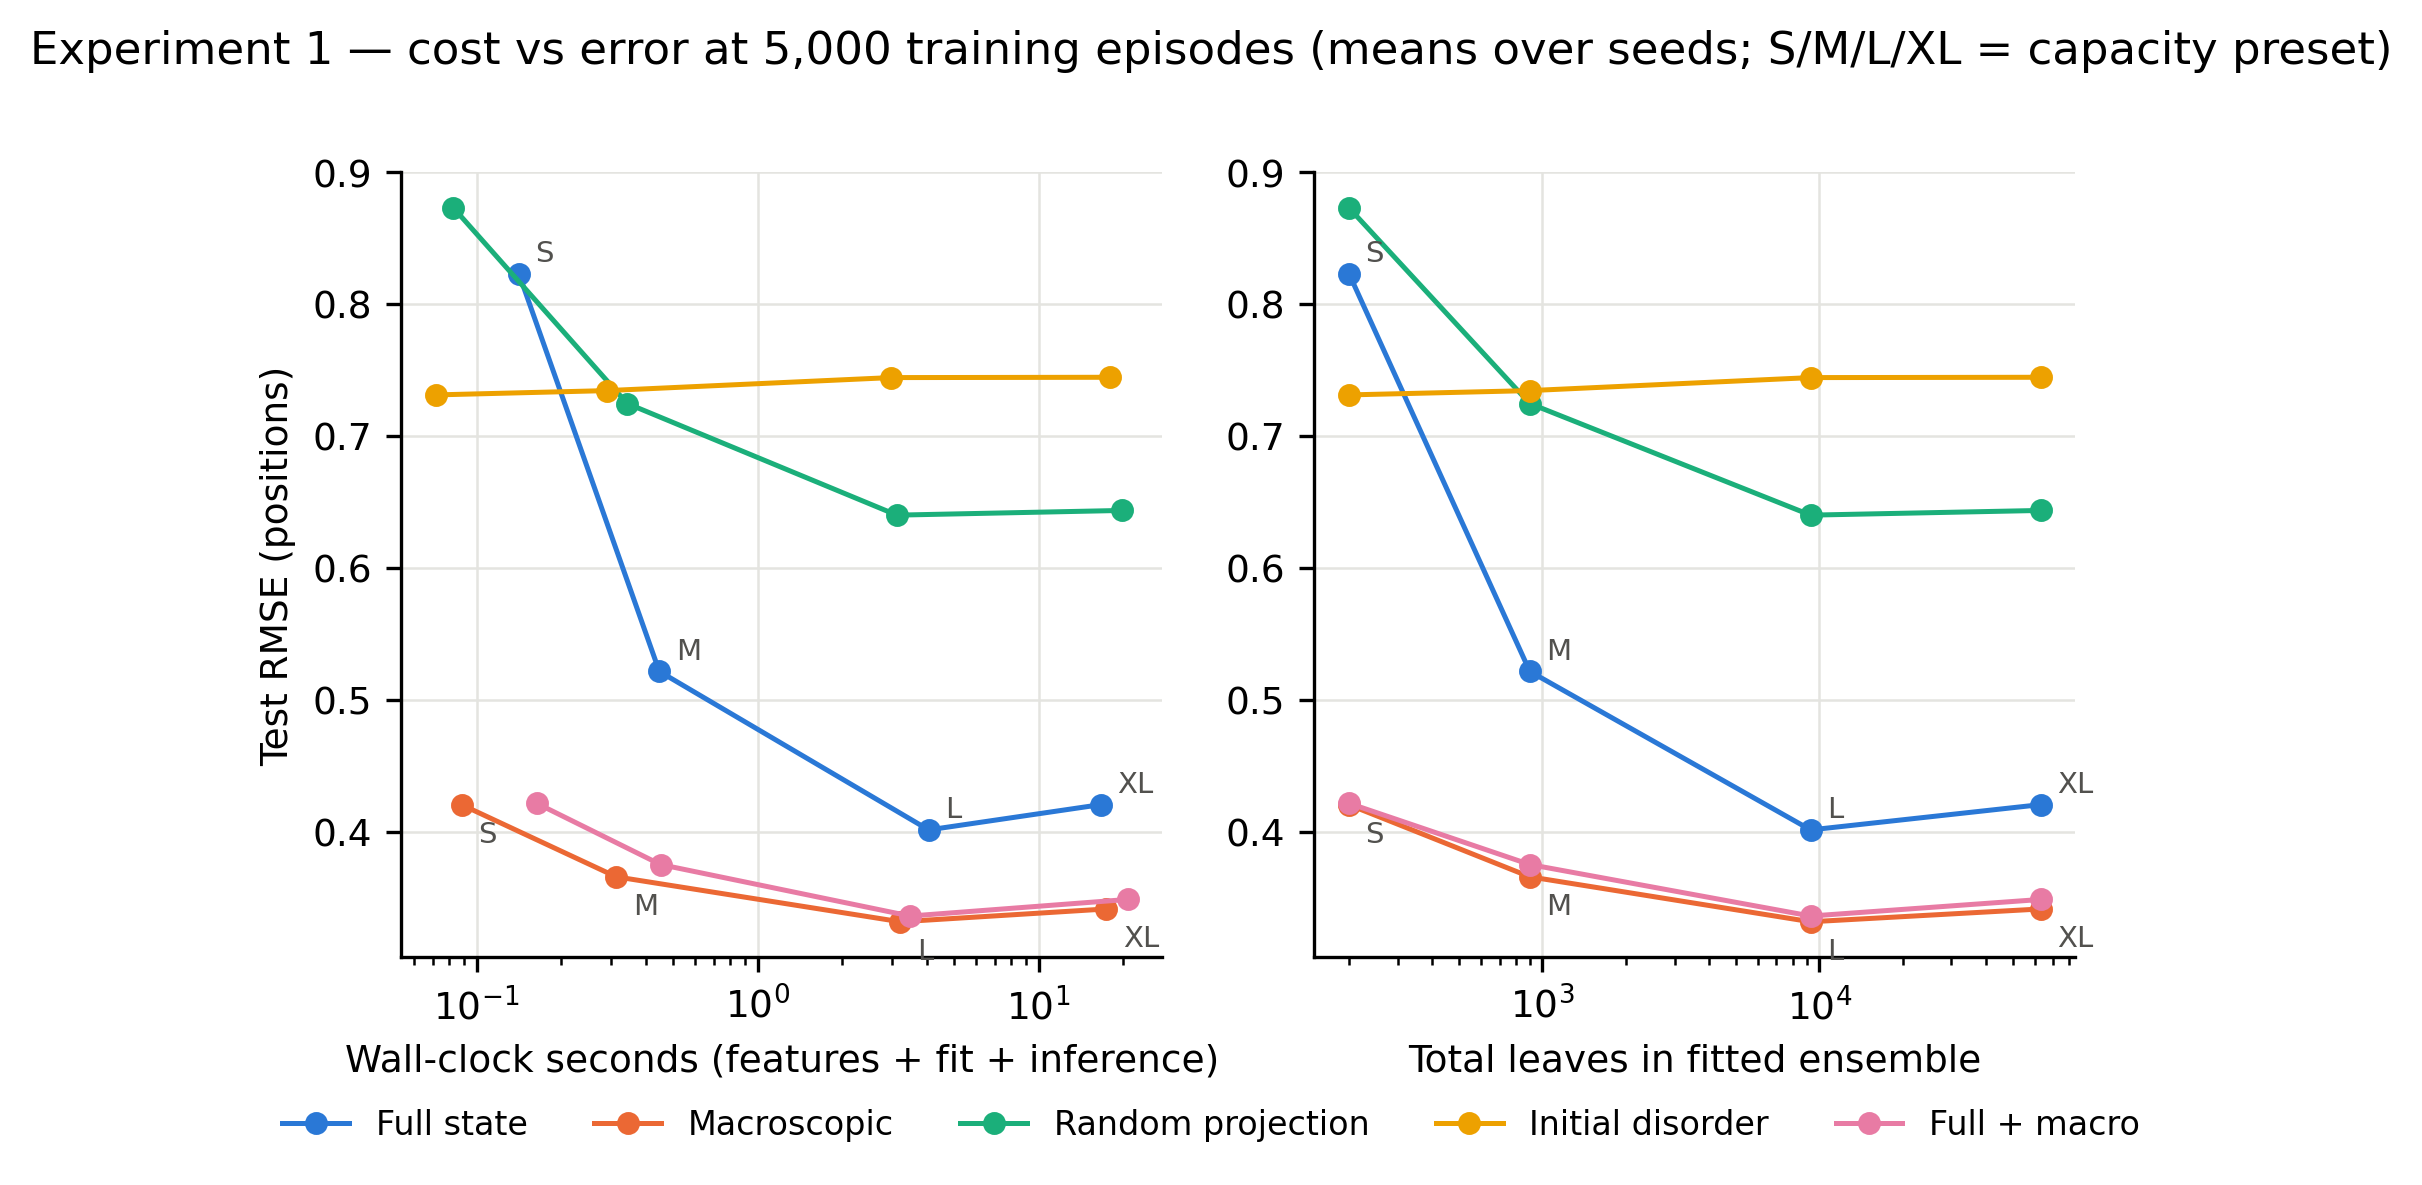
\includegraphics[width=0.9\linewidth]{figures/exp1_cost_vs_error.png}
  \caption{Test RMSE vs.\ total wall-clock cost (left) and realised ensemble
  size (right) at 5,000 episodes; S/M/L/XL mark the capacity presets.}
  \label{fig:cost}
\end{figure}

Costs (Figure~\ref{fig:cost}): feature extraction is negligible (0.4\,ms raw,
2.6\,ms macro, 3.1\,ms projection per 5,000 episodes). Fit time is set by the
preset and secondarily by feature count (medium: 0.44\,s full vs.\ 0.30\,s
macro; large: 4.03\,s vs.\ 3.20\,s). In a measured cost/error comparison, rather than fixed-time
training, macro at medium (0.31\,s, RMSE 0.366) beats full state at large
(4.06\,s, RMSE 0.401) at $13\times$ lower cost.

\begin{figure}[t]
  \centering
  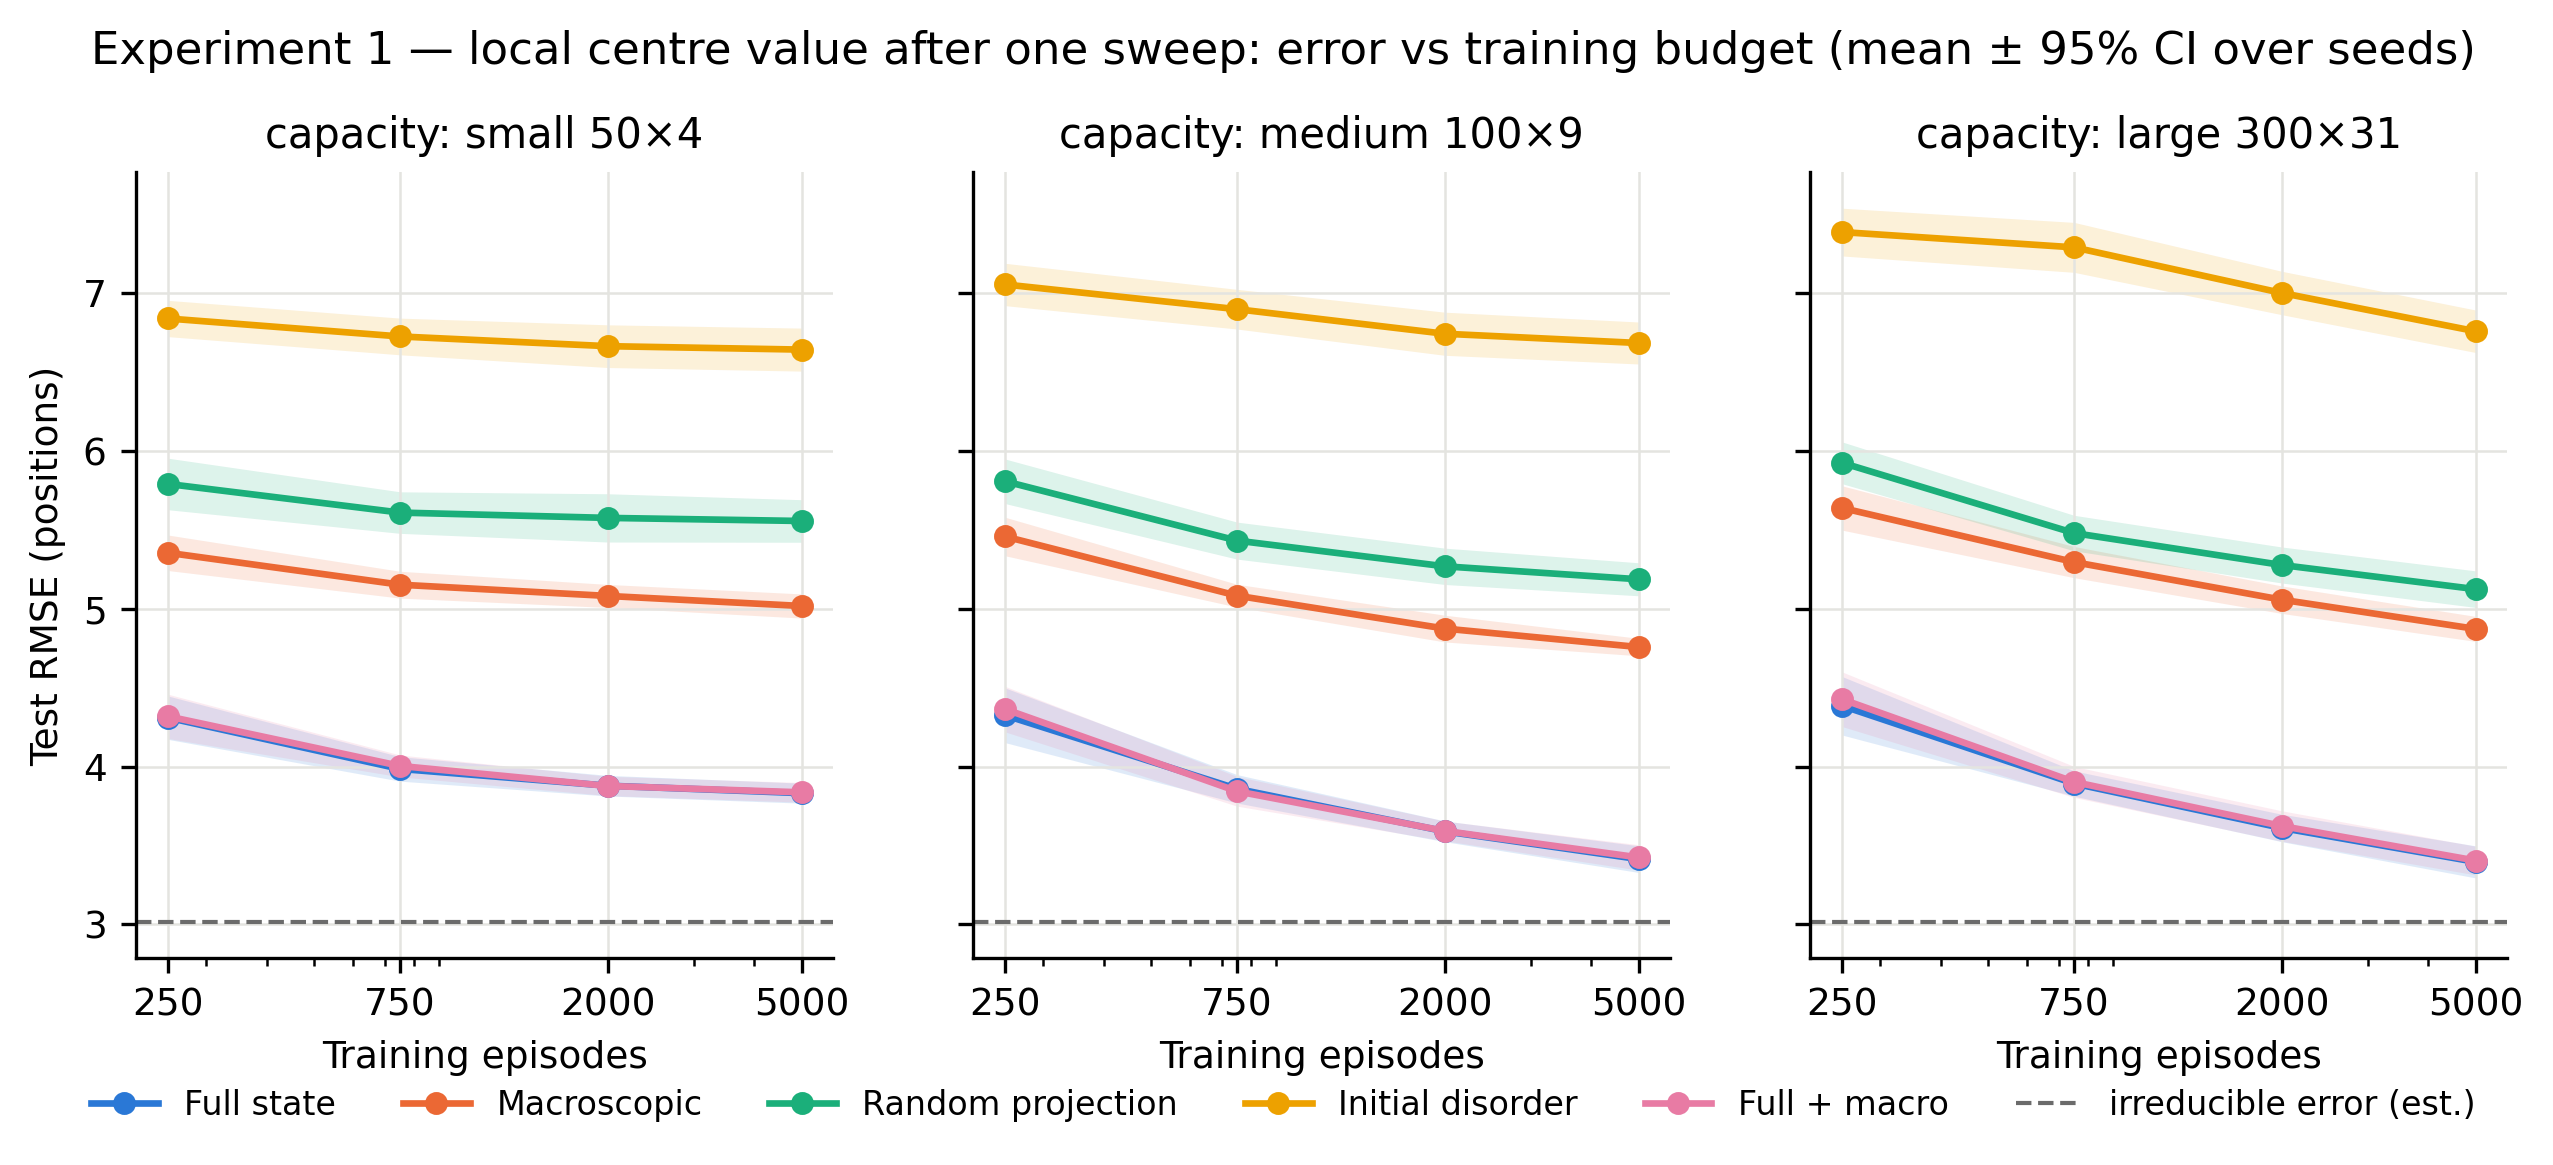
\includegraphics[width=\linewidth]{figures/exp1_local_control.png}
  \caption{Local control task (centre value after one sweep): the ranking
  inverts.}
  \label{fig:local}
\end{figure}

Local control (Figure~\ref{fig:local}; medium/5,000): Full state
$3.413\pm0.118$, Macroscopic $4.757\pm0.077$, Random projection
$5.187\pm0.146$, Initial disorder $6.684\pm0.186$, Full + macro
$3.424\pm0.112$; irreducible 3.01. The full state wins in 10/10 seeds at every
budget and capacity, and its margin grows with capacity ($+24\%$ at small/250
to $+43\%$ at large/5,000).

\subsection{Experiment 2}

\begin{figure}[t]
  \centering
  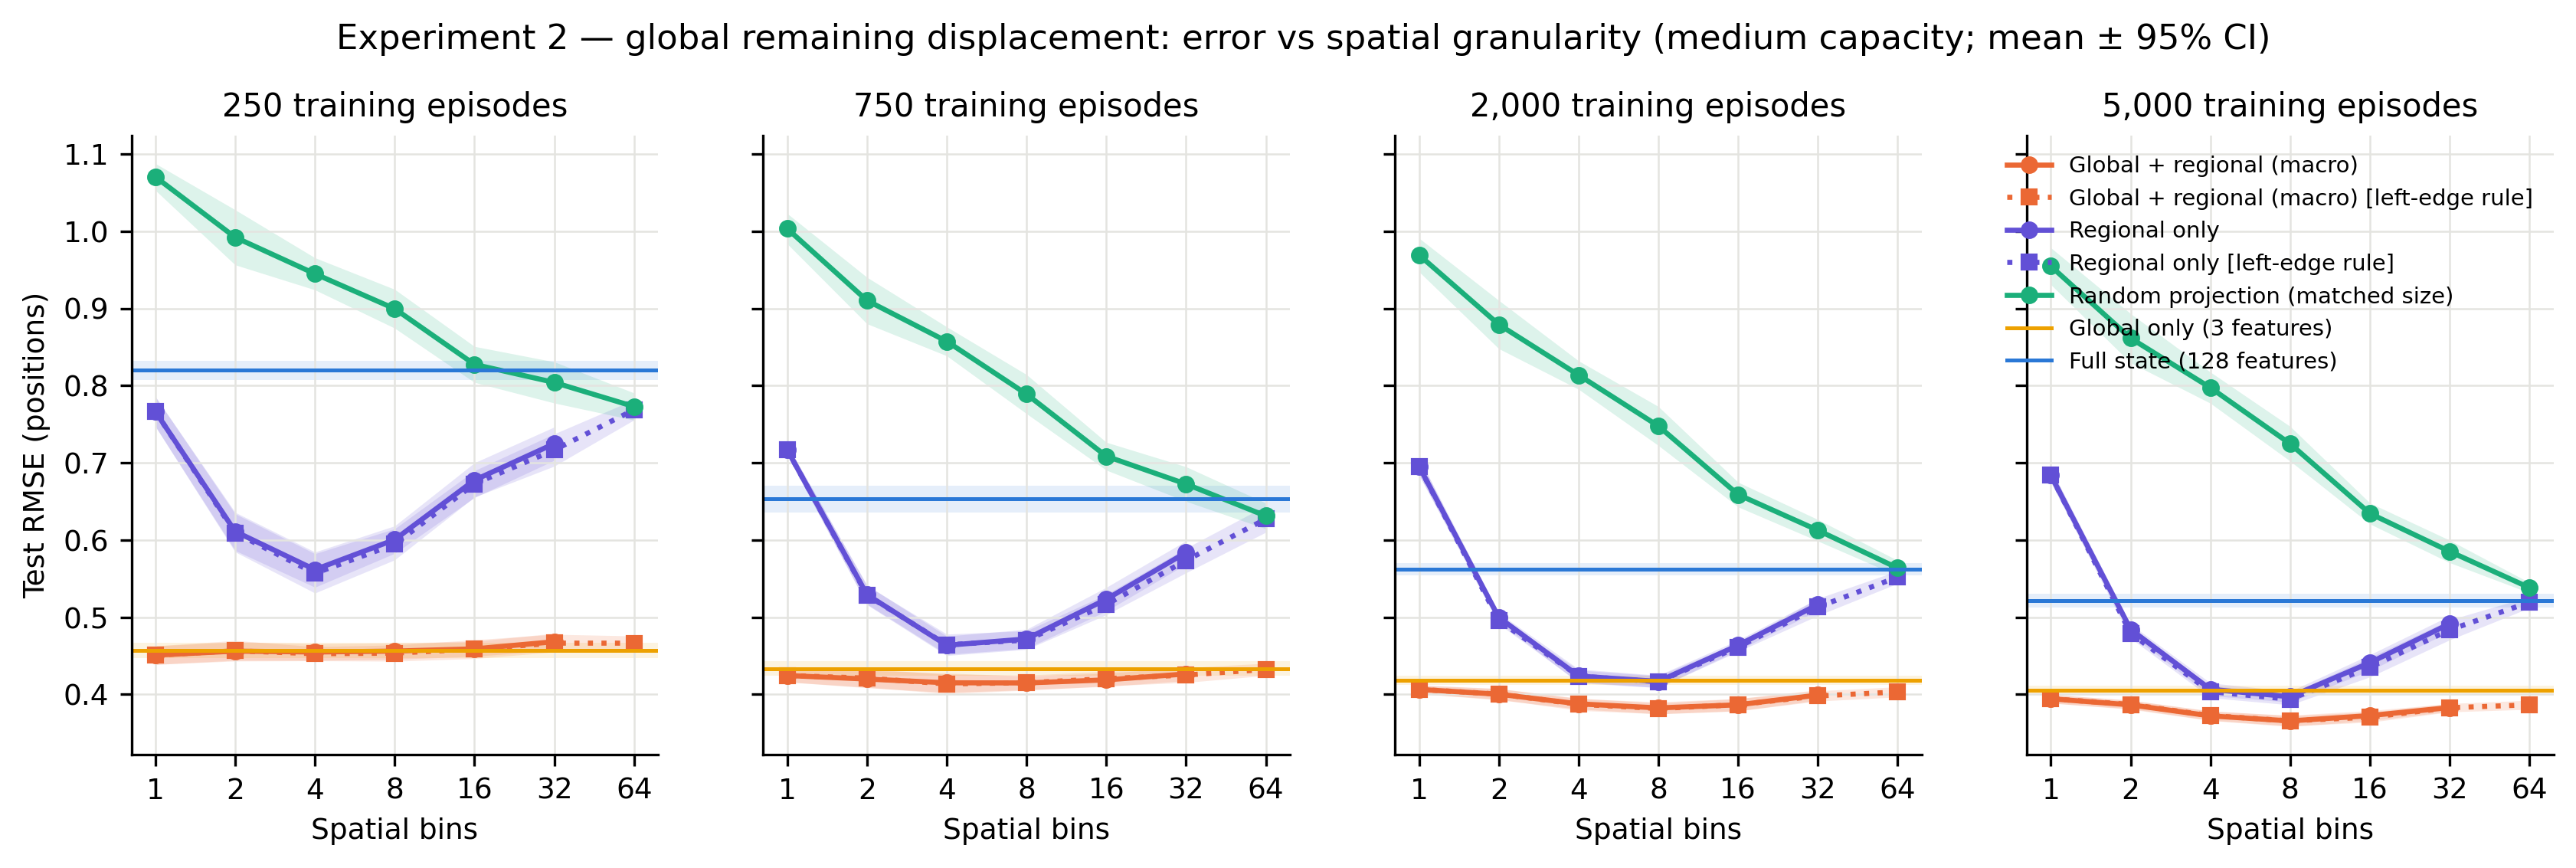
\includegraphics[width=\linewidth]{figures/exp2_error_vs_bins.png}
  \caption{Test RMSE vs.\ number of spatial bins at the medium preset, one
  panel per budget. Lines: macro (global + regional), regional-only,
  dimension-matched random projection; horizontal bands: global-only and raw
  references.}
  \label{fig:bins}
\end{figure}

\begin{table}[t]
\centering
\caption{Test RMSE vs.\ resolution, medium preset, 5,000 episodes (mean $\pm$
SD over 10 seeds; feature counts macro / regional / random).}
\label{tab:exp2}
\begin{tabular}{rlrrr}
\toprule
Bins & Features & Macro & Regional only & Random proj.\\
\midrule
1  & 6 / 3 / 6       & $0.394\pm0.008$ & $0.684\pm0.012$ & $0.955\pm0.033$\\
2  & 9 / 6 / 9       & $0.387\pm0.008$ & $0.484\pm0.009$ & $0.861\pm0.044$\\
4  & 15 / 12 / 15    & $0.372\pm0.008$ & $0.407\pm0.011$ & $0.797\pm0.028$\\
8  & 27 / 24 / 27    & $\mathbf{0.366\pm0.010}$ & $\mathbf{0.397\pm0.010}$ & $0.725\pm0.031$\\
16 & 51 / 48 / 51    & $0.373\pm0.009$ & $0.441\pm0.014$ & $0.634\pm0.019$\\
32 & 99 / 96 / 99    & $0.383\pm0.007$ & $0.492\pm0.014$ & $0.585\pm0.020$\\
64 & 195 / 192 / 195 & $0.387\pm0.008$ & $0.519\pm0.010$ & $0.538\pm0.009$\\
\midrule
global only & 3   & $0.405\pm0.009$ & & \\
raw         & 128 & $0.521\pm0.012$ & & \\
\bottomrule
\end{tabular}
\end{table}

Paired against 8 bins at 5,000 episodes, every other macro resolution is worse:
1 bin $+0.029$ $[0.025,0.032]$, 4 bins $+0.007$ $[0.003,0.011]$, 16 bins
$+0.007$ $[0.004,0.010]$, 32 bins $+0.017$ $[0.014,0.021]$, 64 bins (left
rule) $+0.021$ as a difference of means; global-only $+0.040$ $[0.037,0.042]$;
raw $+0.156$ $[0.142,0.170]$. Eight bins is the validation-best resolution in
8/10 seeds (4 bins in the other two). At 250 episodes, by contrast, no
resolution differs detectably from 8 bins except 32 ($+0.012$), the whole sweep
lies within 0.451--0.468, and 1 bin is the validation-best choice in 4/10 seeds
(7/10 at the small preset).

\begin{figure}[t]
  \centering
  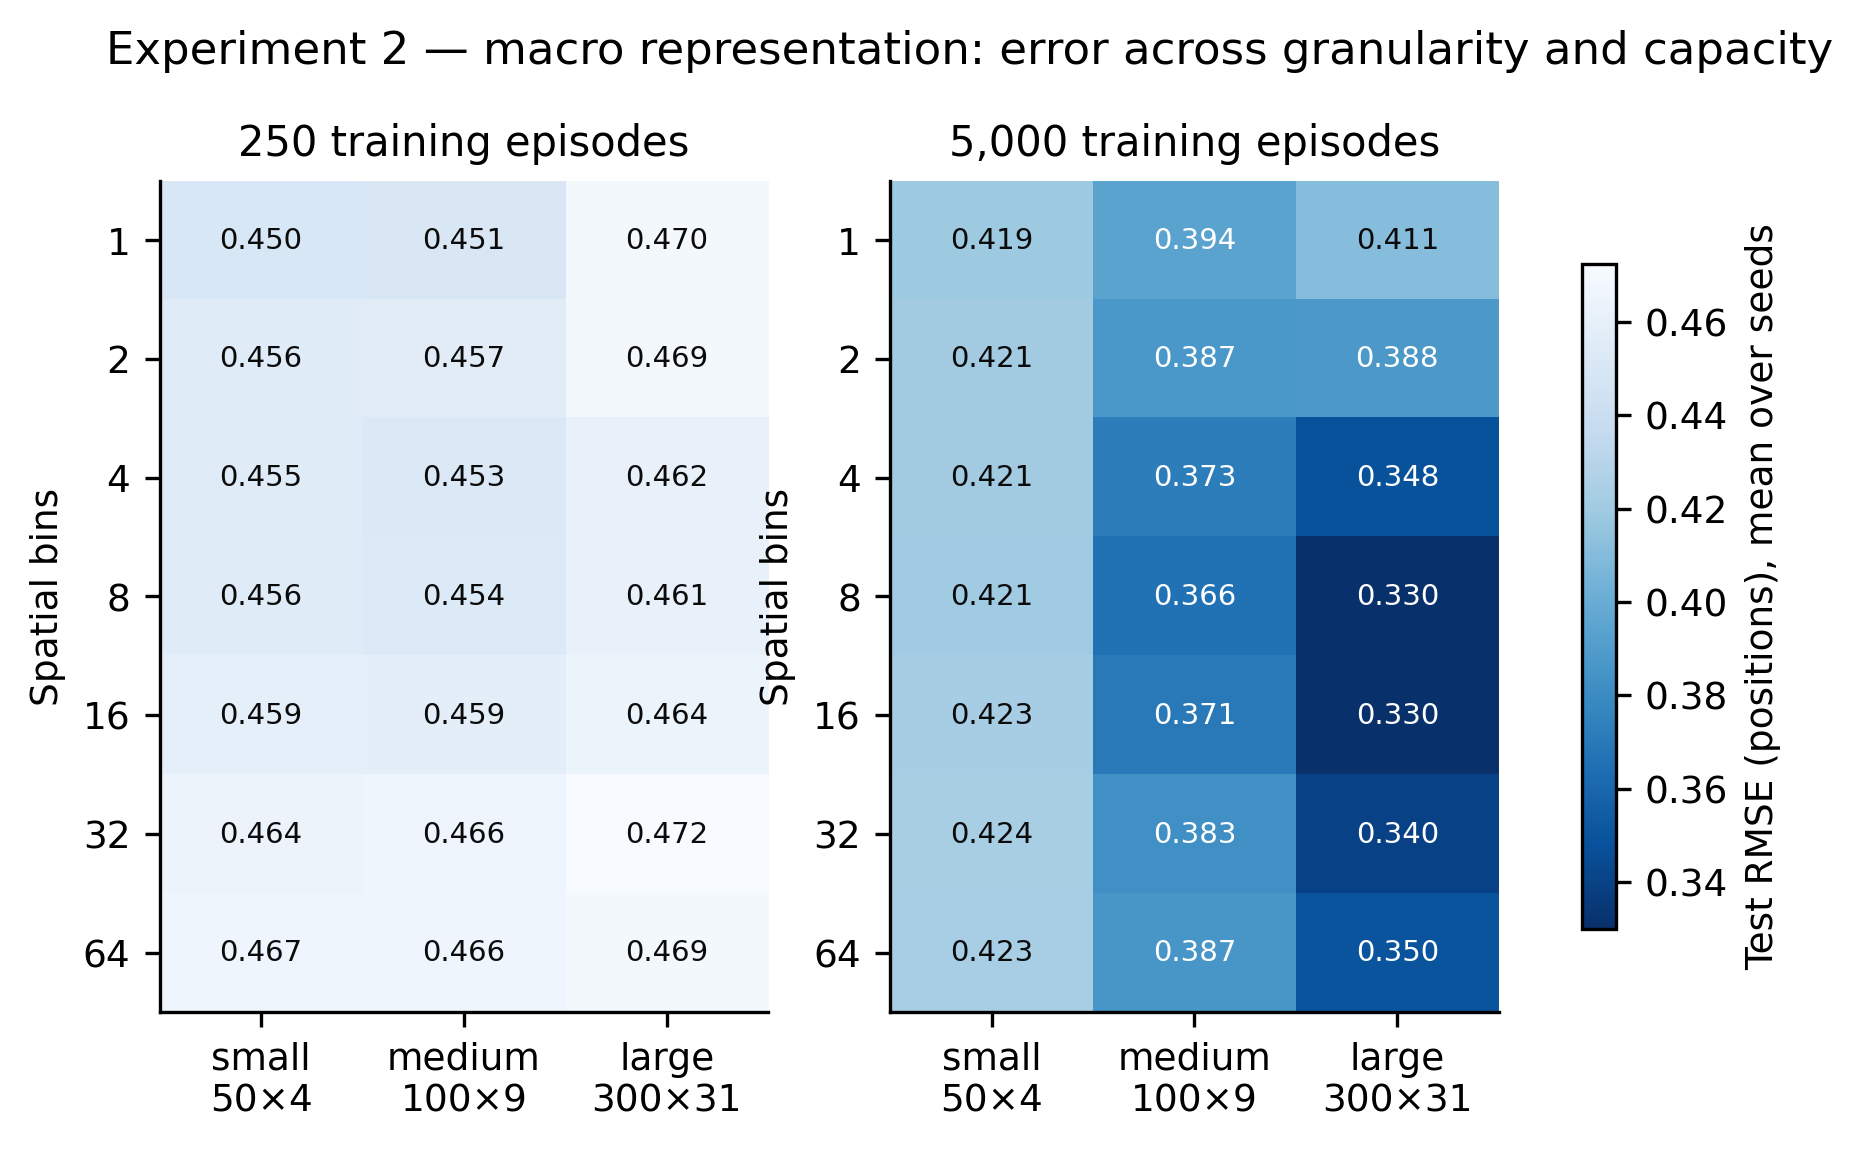
\includegraphics[width=0.85\linewidth]{figures/exp2_heatmap.png}
  \caption{Macro test RMSE across resolution and capacity at 250 and 5,000
  episodes.}
  \label{fig:heatmap}
\end{figure}

Granularity $\times$ capacity (Figure~\ref{fig:heatmap}): at 250 episodes
every cell lies in 0.450--0.472. At 5,000, the small preset is flat
(0.419--0.424), medium is minimal at 8 bins, and large is minimal at 8--16 bins
(0.330 / 0.330; 1 bin 0.411, 64 bins 0.350). The optimal resolution moves finer
as resources grow.

\begin{figure}[t]
  \centering
  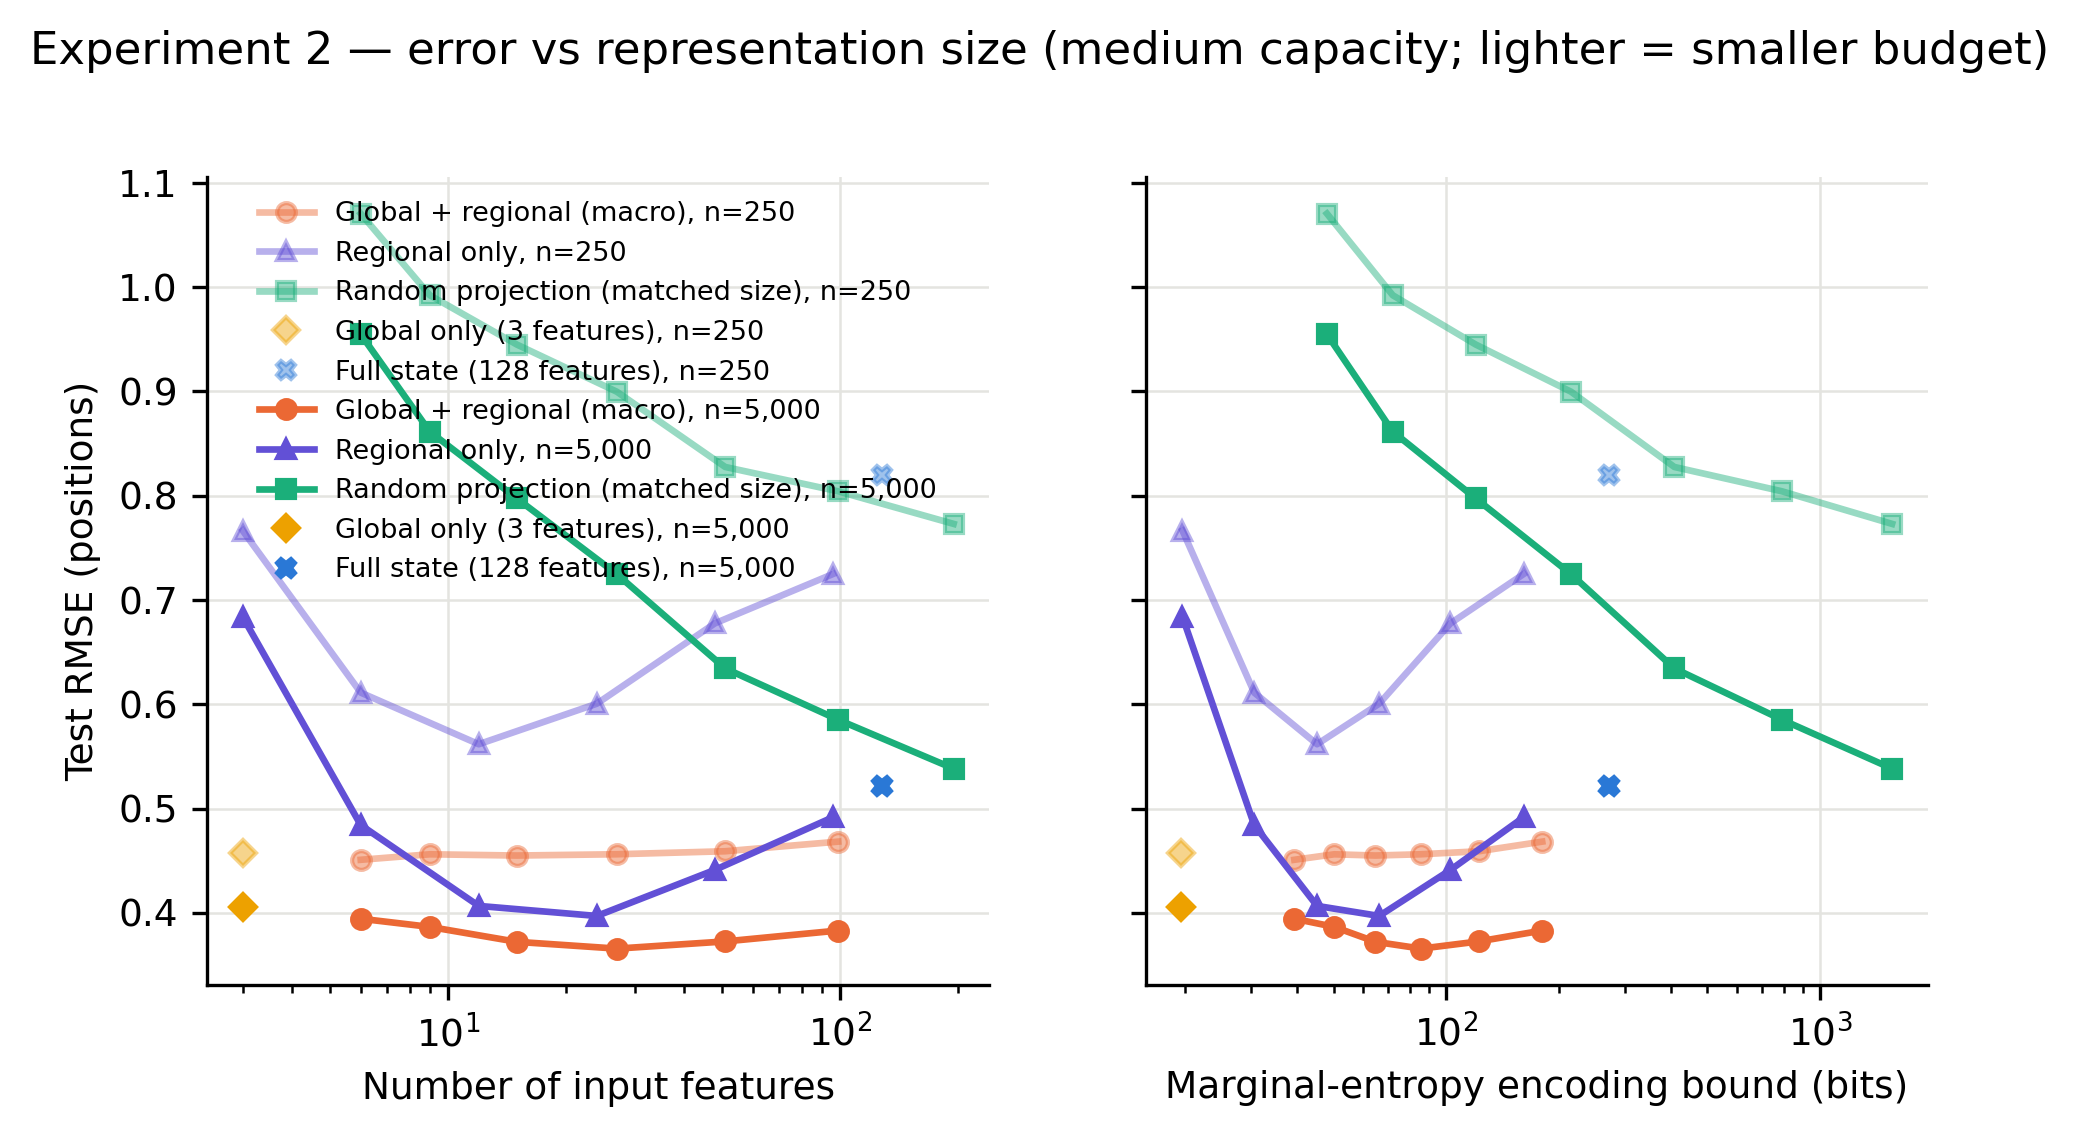
\includegraphics[width=0.9\linewidth]{figures/exp2_error_vs_size.png}
  \caption{Test RMSE vs.\ feature count (left) and marginal-entropy encoding
  bound (right).}
  \label{fig:size}
\end{figure}

Ablations (Figure~\ref{fig:size}): the three global statistics alone reach
0.405, about 11\% above the best medium model and 0.12 better than the raw state. The
regional-only series has a pronounced interior optimum (0.684 at 1 bin, 0.397
at 8, 0.519 at 64). Permutation importance of the 8-bin model is dominated by
the displacement $\times$ unreliability interaction ($0.932\pm0.030$ RMSE
increase when permuted) and mean displacement ($0.130\pm0.013$); every regional
feature contributes $\le0.01$. The random projection improves monotonically with
dimension and reaches the raw state's level only at 195 dimensions. The 64-bin
macro representation has a larger entropy bound (314 bits) than the raw state
(273 bits) yet 26\% lower error.

\begin{figure}[t]
  \centering
  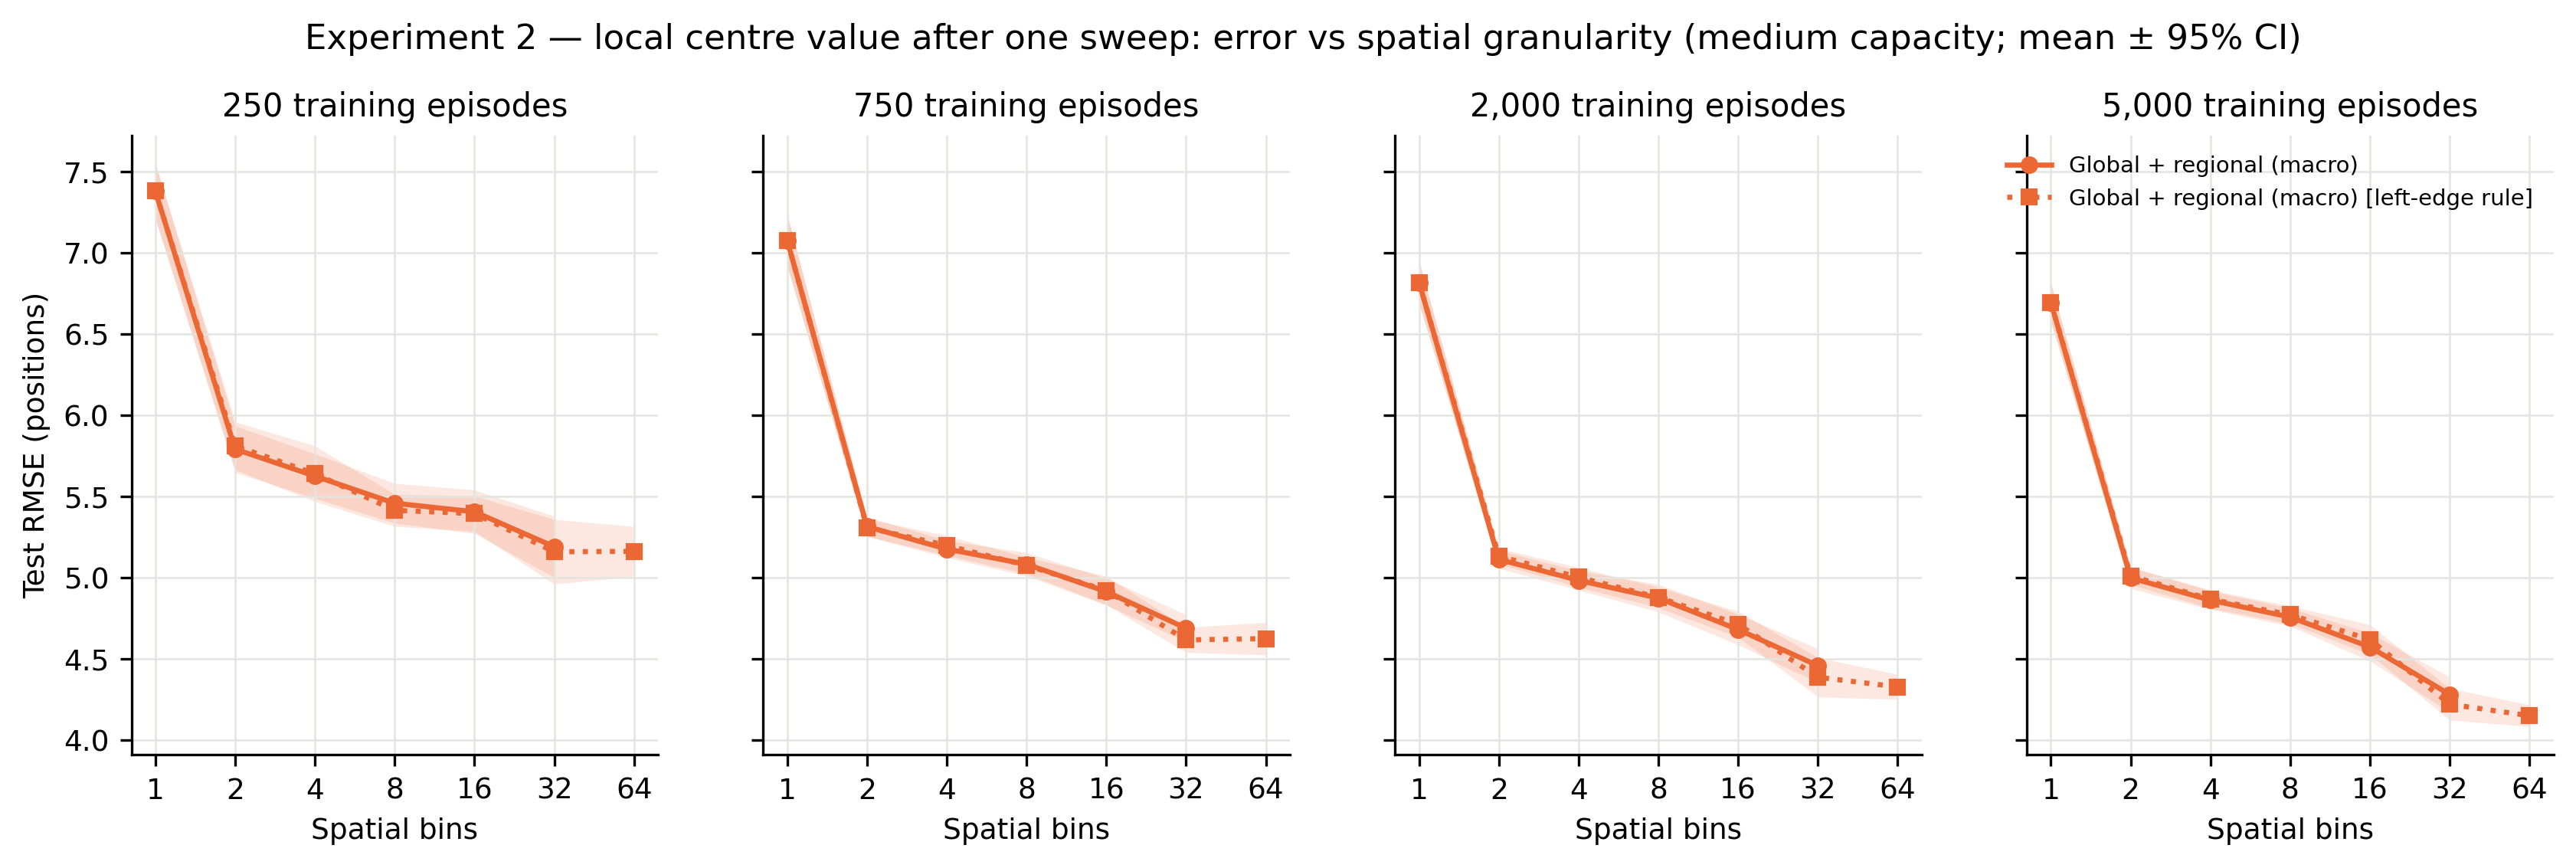
\includegraphics[width=\linewidth]{figures/exp2_local_vs_bins.png}
  \caption{Local control task vs.\ resolution: finer is monotonically better.}
  \label{fig:localbins}
\end{figure}

Local control (Figure~\ref{fig:localbins}; macro, medium, 5,000): 6.70 at 1
bin, 4.76 at 8, 4.15 at 64; 32 or 64 bins is validation-best in 10/10 seeds;
all remain far above the raw state (3.41). Costs grow mildly with feature count
(fit 0.19--0.27\,s for engineered sets vs.\ 0.32\,s raw and 0.47\,s for the
195-dimensional projection; extraction $\le3.7$\,ms).

\subsection{Experiment 2b}\label{sec:exp2b-results}

\begin{figure}[t]
  \centering
  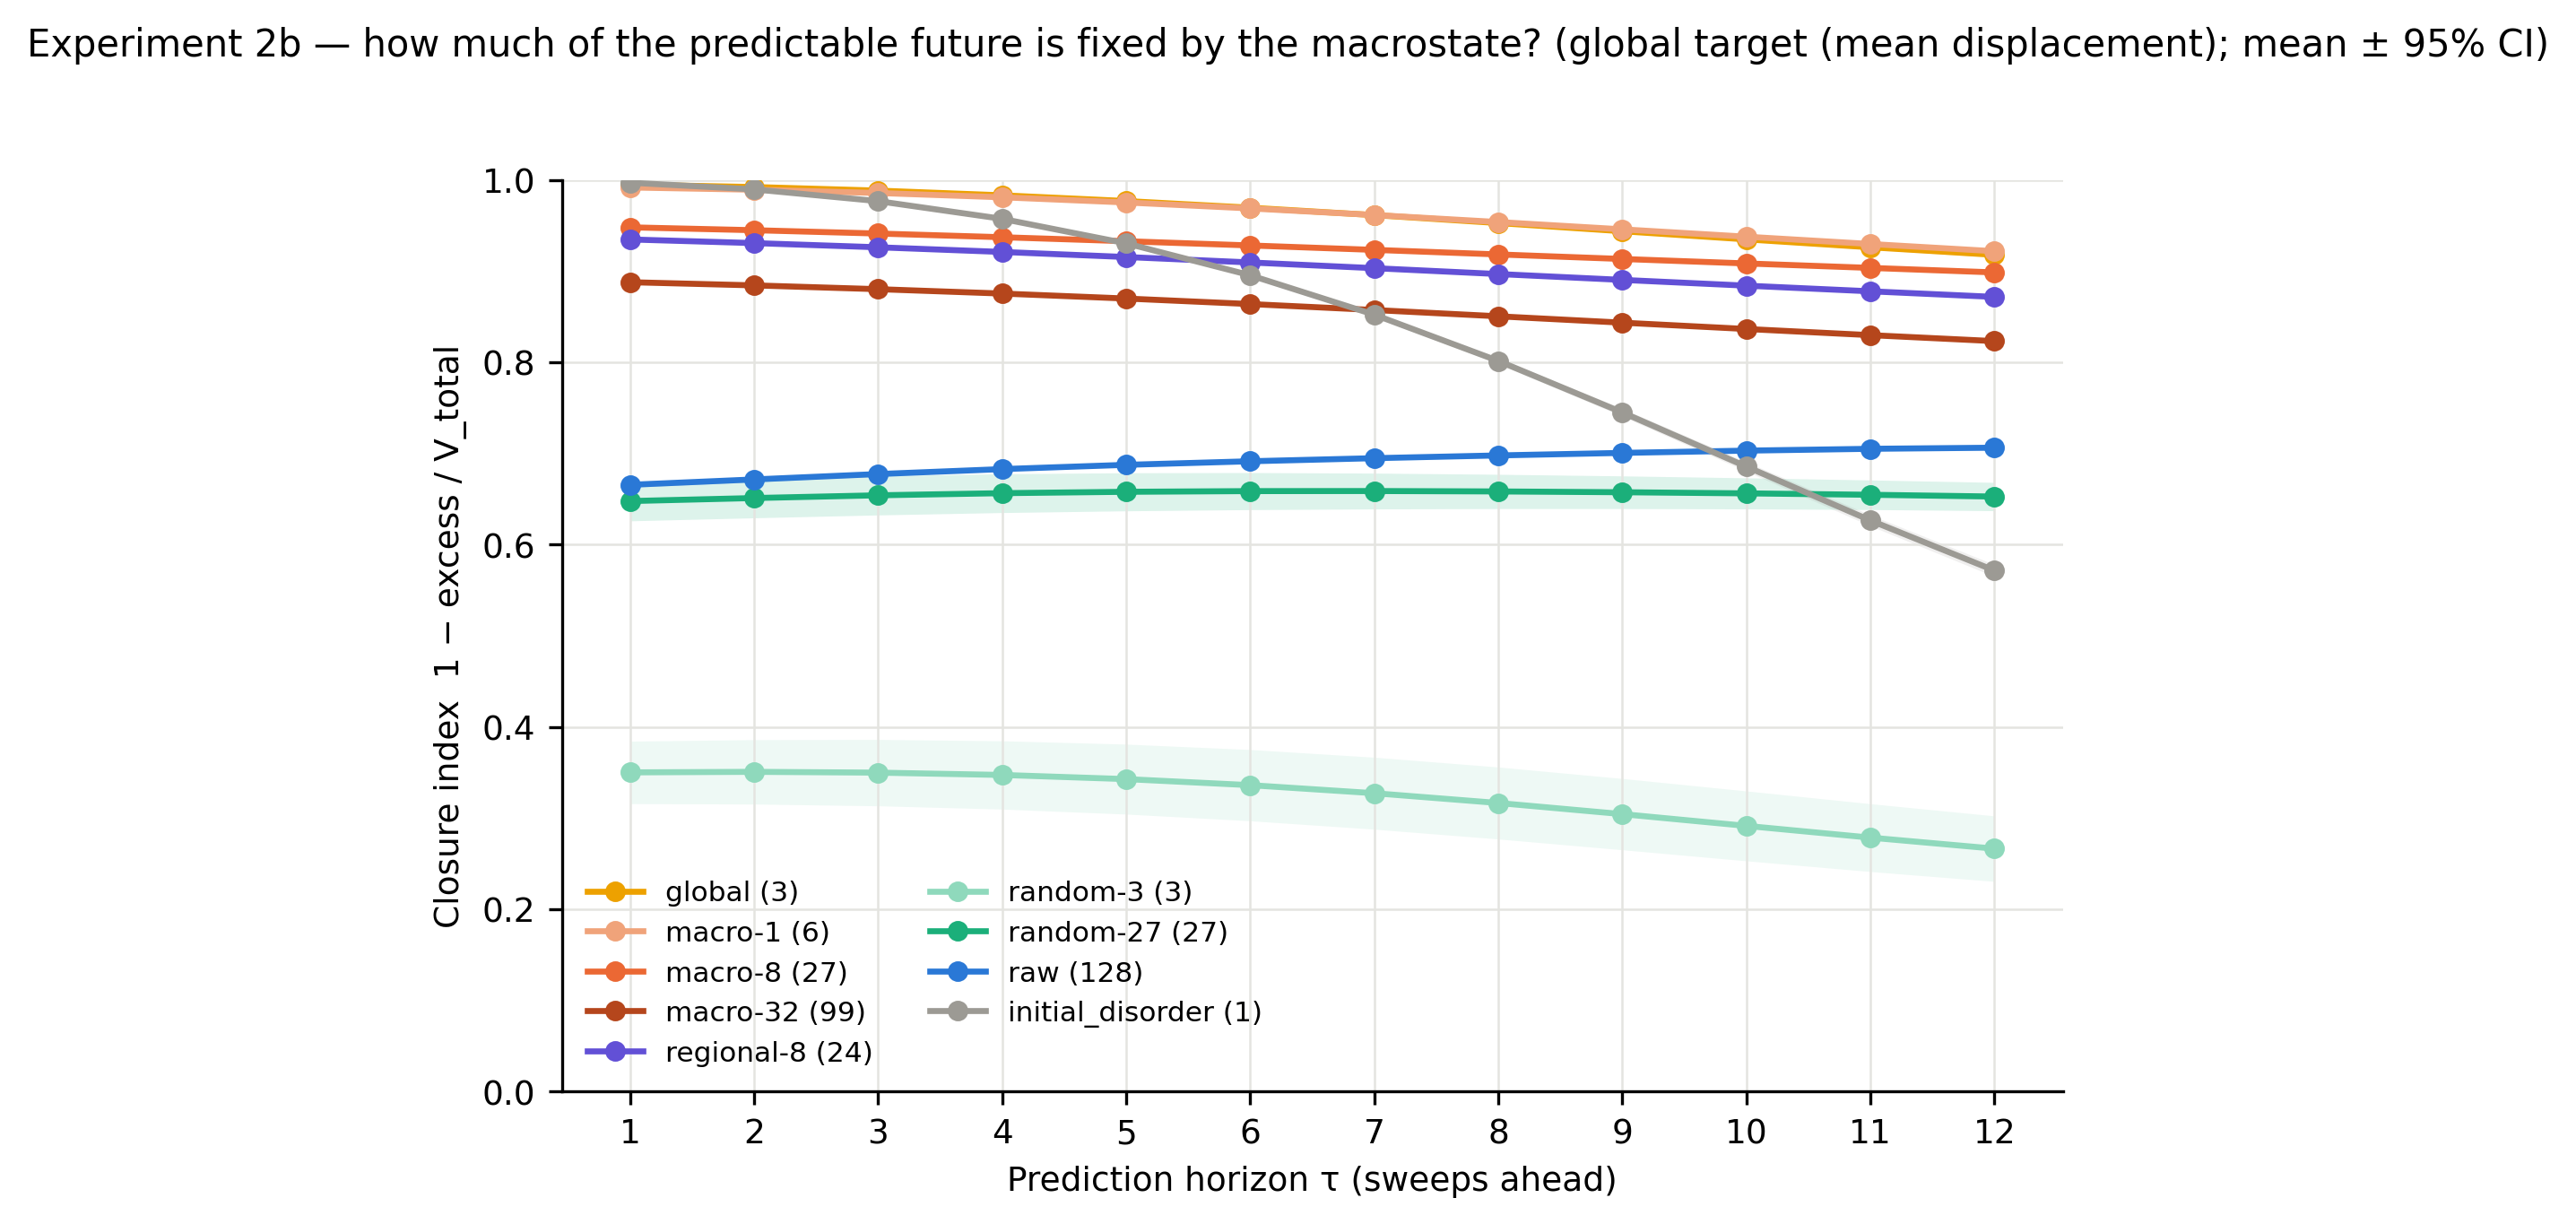
\includegraphics[width=0.9\linewidth]{figures/exp2b_closure_vs_horizon.png}
  \caption{Closure index vs.\ prediction horizon for the global target (mean
  $\pm$ 95\% CI over 10 seeds). A value of 1 means configurations matched on
  the abstraction have identical conditional-mean futures.}
  \label{fig:closure}
\end{figure}

\begin{table}[t]
\centering
\caption{Closure index at $\tau=12$ (target), 10,000 configurations, mean over
10 seeds (SD $\le0.004$ unless shown).}
\label{tab:closure}
\begin{tabular}{lrrrr}
\toprule
Abstraction & Features & Rel.\ nbr.\ distance & Closure & Matched-size random proj.\\
\midrule
Initial disorder & 1   & 0.001 & 0.572 & \\
Global           & 3   & 0.040 & \textbf{0.918} & 0.266 ($\pm0.06$)\\
Macro-1          & 6   & 0.082 & 0.922 & 0.449\\
Macro-8          & 27  & 0.292 & 0.899 & 0.653\\
Regional-8       & 24  & 0.296 & 0.872 & \\
Macro-32         & 99  & 0.470 & 0.823 & 0.686\\
Raw state        & 128 & 0.460 & 0.706 & \\
\bottomrule
\end{tabular}
\end{table}

Configurations matched on the three global summaries, at a relative neighbour
distance of 0.04, have futures twelve sweeps ahead whose true conditional
means agree to within 8\% of their variance ($V_{\text{total}}=1.199\pm0.025$
positions$^2$; $V_{\text{irr}}=0.031$). Paired against controls: global $-$
random-3 $=+0.652$ $[0.614,0.689]$; macro-8 $-$ random-27 $=+0.246$
$[0.230,0.262]$; global $-$ initial disorder $=+0.347$ $[0.339,0.354]$; all
10/10 seeds. Measuring the future by the three global summaries instead of the
target gives global closure 0.929 and initial disorder 0.545. Closure of the
global summaries falls slowly with horizon (0.995 at $\tau=1$); the disorder
scalar is almost closed at $\tau=1$ (0.997) and collapses to 0.572 by
$\tau=12$, because the long-horizon recovery depends on where the disorder sits
relative to the unreliable region, which only the interaction feature carries.

\begin{figure}[t]
  \centering
  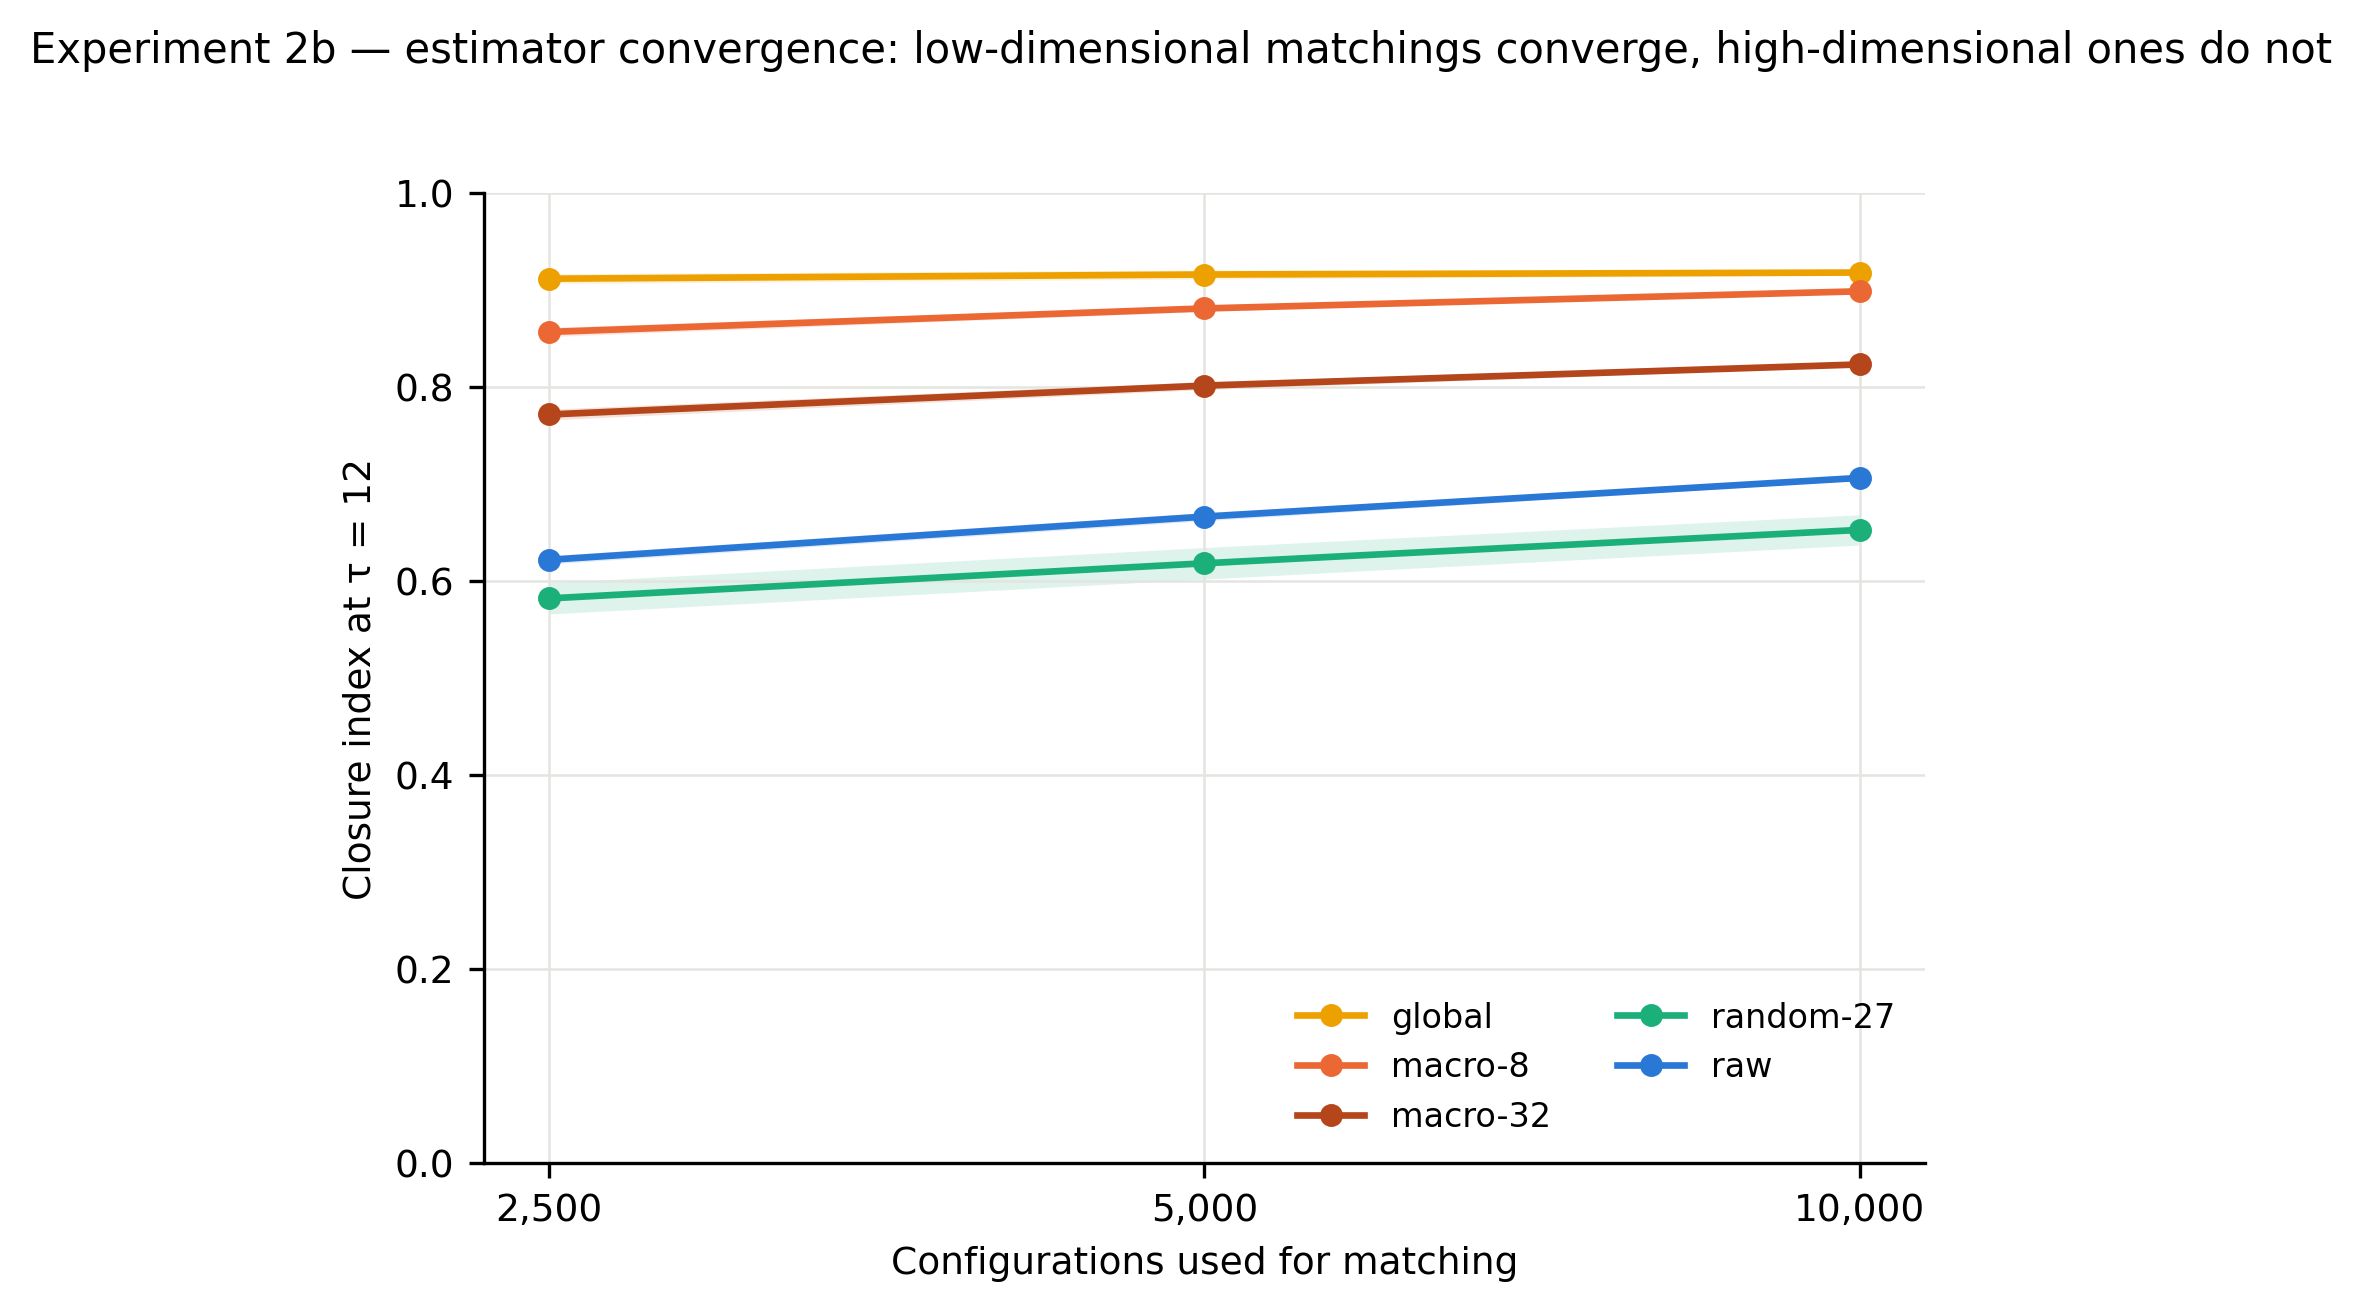
\includegraphics[width=0.75\linewidth]{figures/exp2b_convergence.png}
  \caption{Estimator convergence with the number of configurations.}
  \label{fig:convergence}
\end{figure}

The global estimate changes relatively little over the tested sample sizes
($0.912\to0.916\to0.918$ at $2{,}500\to5{,}000\to10{,}000$); the
higher-dimensional estimates are still rising (macro-8
$0.857\to0.881\to0.899$; raw $0.622\to0.666\to0.706$;
Figure~\ref{fig:convergence}). This indicates downward matching bias,
particularly at high dimensionality, rather than establishing rigorous lower
bounds or complete convergence. Matched-size controls reduce, but do not
eliminate, geometric differences between representations.

\begin{figure}[t]
  \centering
  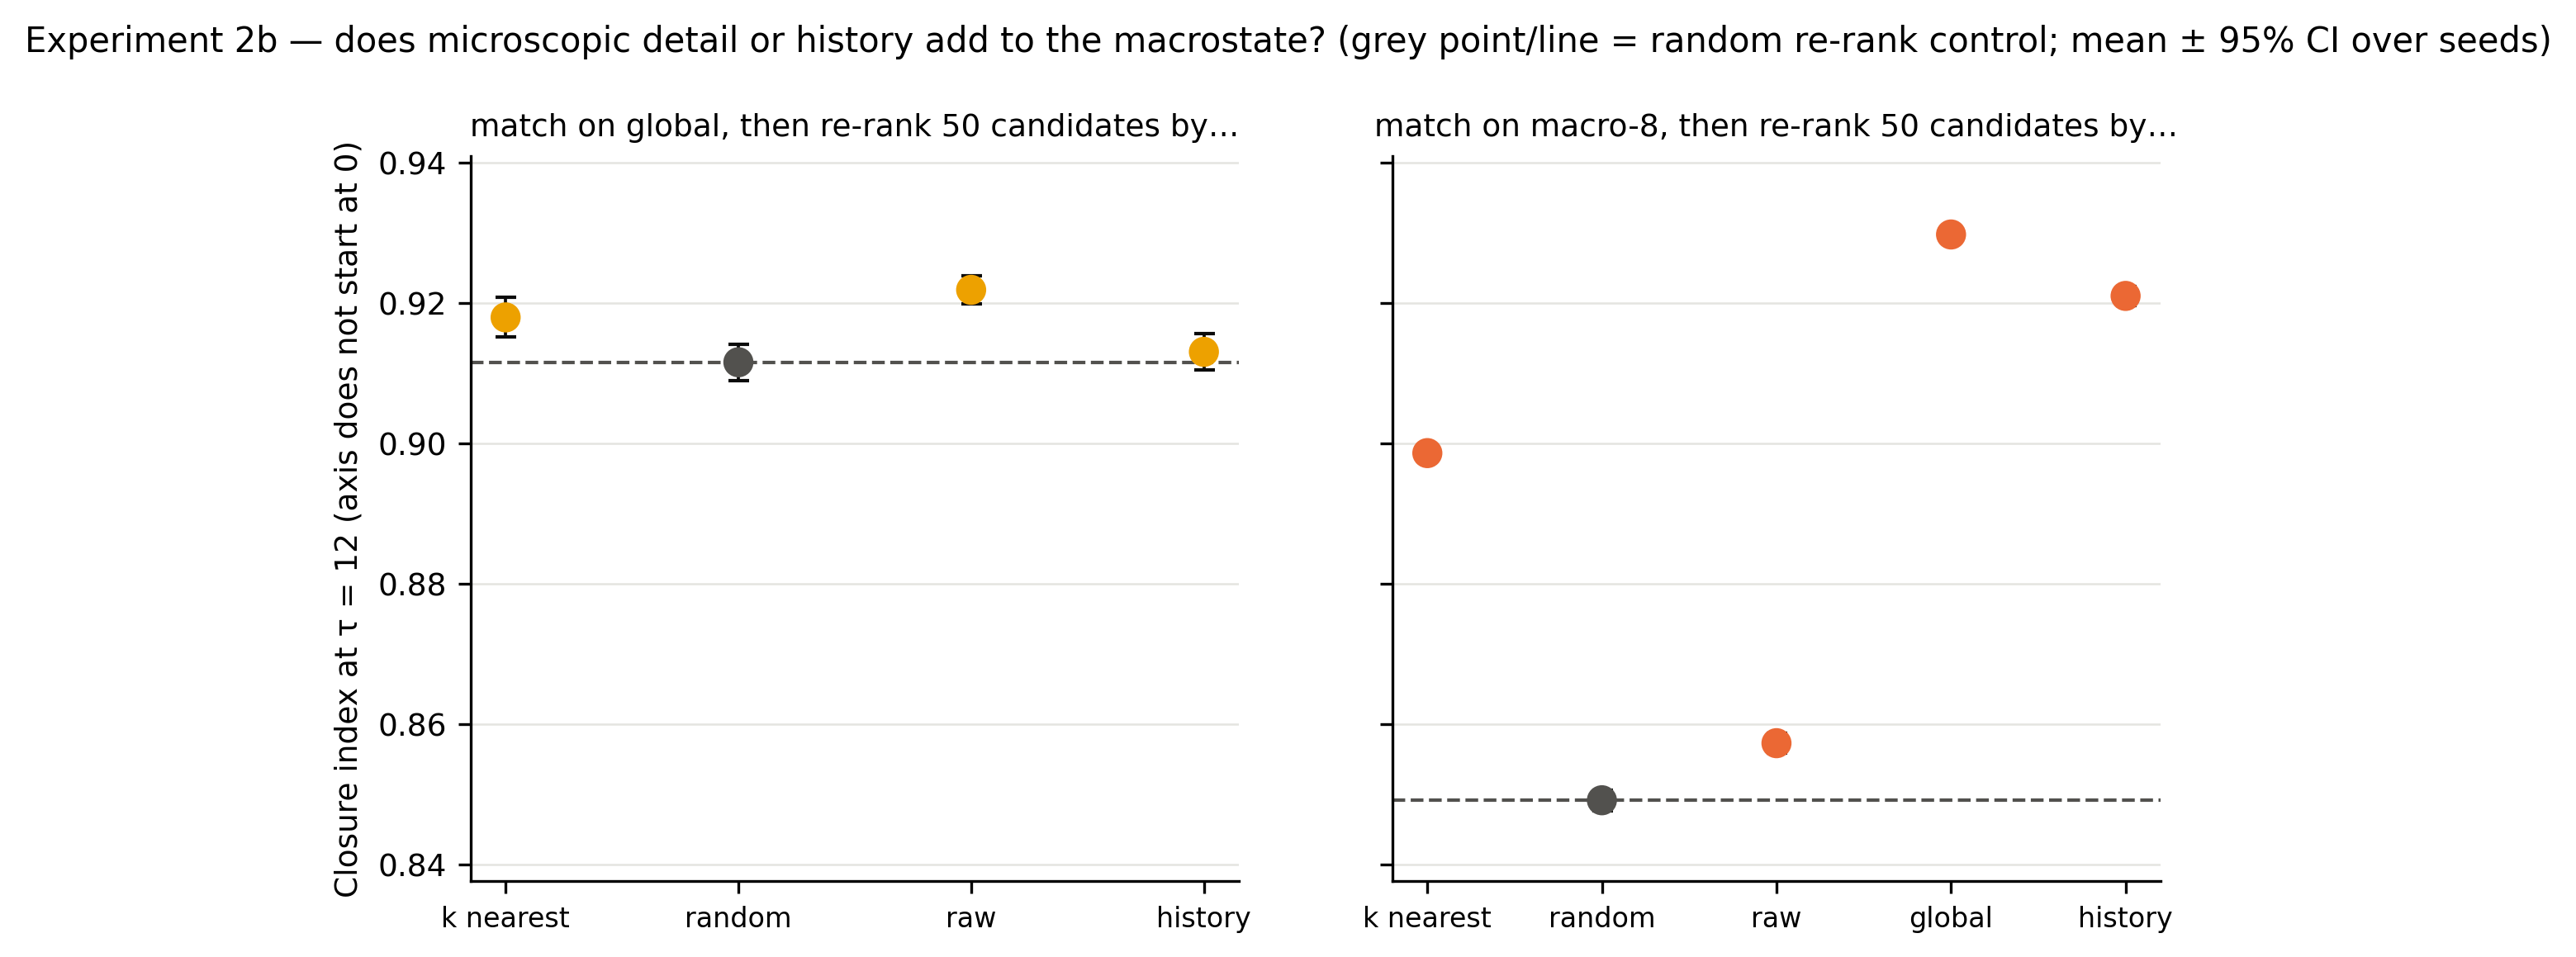
\includegraphics[width=0.95\linewidth]{figures/exp2b_refinements.png}
  \caption{Closure after re-ranking the 50 nearest macro-neighbours by
  raw-state distance, by the previous sweep's global summaries, by the present
  global summaries, or at random.}
  \label{fig:refinements}
\end{figure}

Re-ranking the global-matched candidates by raw-state distance raises closure
by $+0.0103$ $[0.0094,0.0112]$ over the random re-rank control (10/10 seeds);
re-ranking by the previous macrostate raises it by $+0.0015$
$[0.0005,0.0025]$. At the macro-8 level, present-global re-ranking ($+0.081$
over random) does as much as history re-ranking ($+0.072$), and history is
slightly worse than present-global ($-0.009$ $[-0.009,-0.008]$): this comparison is consistent with improved present-state matching
rather than evidence for a large history effect, but it does not rule out
dependence on a longer or richer past
(Figure~\ref{fig:refinements}).

\section{Discussion}\label{sec:discussion}

Throughout this section we distinguish \textbf{established findings}
(reproducible results of the previous section or theorems),
\textbf{interpretations} (our explanations of them), \textbf{hypotheses}
(mechanisms not yet tested) and \textbf{inspirations} (ideas that motivate the
programme without being evidence for it).

\subsection{The baseline finding survives, in a qualified form (finding and interpretation)}
Ten seeds, four capacities and validation-based selection all agree that the
engineered macroscopic representation lowers the error a gradient-boosting
learner attains on the global target, consistently across all 130 tested
seed $\times$ budget $\times$ capacity cells. But the size of the effect is a
strong function of resources: it is roughly halved error at 250 episodes and a
17\% reduction at 5,000 episodes with the larger model. The raw-state curve has
not converged, and both curves sit far above the noise floor, so the data are
consistent with a declining gap, motivating larger-budget tests. The
Bayes-risk ordering does not guarantee that this particular learner will
converge to an optimal representation. The claim supported is therefore not that the summary is better in an
absolute sense but that it buys a large head start for a bounded learner, a head
start that is worth more when the learner is more constrained and is
also visible in the measured cost/error comparison.

\subsection{It is the content, not the compression (finding and interpretation)}
Three results separate the effect of \emph{what} is kept from the effect of
\emph{how much} is kept. The dimension-matched random projection has higher mean error than the raw
state and engineered summary at every tested Experiment~1 setting. It loses
to the disorder scalar at the smallest budget but not in every setting. Three
global numbers capture most of the benefit, and one engineered interaction
carries most of the predictive weight. And a 195-feature engineered
representation with a larger marginal-entropy encoding bound than the raw state still beats it by
a wide margin. A reading of these experiments as evidence that ``throwing
information away'' helps would be wrong; the engineered features re-express the
state in coordinates (displacement relative to the known goal configuration,
unreliability where displaced elements sit) in which the target is a simple
function. In the vocabulary of the Introduction, this is the difference between
compression and abstraction, and the data come down on the side of abstraction:
the useful representations are those that preserve the \emph{relationship}
between misplaced elements and unreliable edges, whatever their size.

\subsection{Coarse-graining has a real but modest, resource-dependent effect (finding and interpretation)}
With the global features present, the resolution sweep shows a shallow interior
optimum at 8--16 bins that is absent at 250 episodes and moves finer as data and
capacity grow, the pattern expected from a bias--variance trade-off. The
regional-only ablation shows the same trade-off in sharper form: 64-bin
features use more coordinates than 8-bin features and give higher mean error
at every tested budget. No strict mutual-information ordering was measured. This is the one place where ``less is more''
holds in its literal sense, and it holds for a bounded learner on a fixed
budget, not for information content.

\subsection{Task dependence and the limits of compression (finding, interpretation and counterargument)}
The local target reverses every ranking: the raw state wins in every seed, the
finest resolution is best, and the raw state's margin grows with capacity. A
representation is useful relative to a prediction target, and no amount of
resource gives the macro summary back the element identities it discarded. This
is the empirical form of a general counterargument to any ``less is more''
thesis. Not every target admits a compact representation; some outcomes depend
irreducibly on microscopic detail (here, which element sits next to which); and
even when a compact law exists, prediction from it can be expensive, as chaos
and computational irreducibility illustrate \citep{wolfram1985}. The same point
separates \emph{possessing} a representation of a problem from \emph{solving}
it efficiently; complexity theory makes the distinction precise
\citep{aaronson2013}, but nothing here bears on asymptotic complexity or on P
versus NP. What our experiments show is only that a good representation can
make structured instances easier for a practical learner under practical
budgets. There is no universally optimal representation in our system, and we
see no reason to expect one elsewhere. The hypothesis we are pursuing is
therefore not that less information is better, but that a capable system must
determine \emph{which} distinctions matter for the task at hand and spend its
limited resources on those, keeping full detail, keeping a summary, or keeping
several levels at once as the task requires. Whether abstraction is \emph{the}
central mechanism of intelligence or one of several interacting mechanisms
(search, memory, exploration, planning, feedback-driven learning) is an open
question that our data do not address; the local task is a reminder that a
system that only abstracts would be as handicapped as one that only remembers.

\subsection{From predictive coarse-graining to abstraction-based intelligence (interpretation and hypothesis)}
Why should an improvement in resource-bounded prediction from supplied features
motivate research into autonomous abstraction? Because it establishes the first
link in a chain and measures its size. The progression we have in mind is:
\begin{enumerate}[1.]
\item \textbf{Useful supplied abstraction.} A representation designed with
  task knowledge reduces the data and compute a learner needs.
  \emph{Investigated here}: the effect exists, is large under scarcity, shrinks
  with resources, is driven by content rather than size, and is task-specific.
\item \textbf{Autonomous abstraction discovery.} A system constructs such a
  representation from raw observations without being told which features
  matter. \emph{Not investigated.} The ablations sharpen what success would
  look like: a learned three-dimensional bottleneck that reached the
  global-only error of 0.405 at 5,000 episodes, and whose coordinates were
  linearly readable as displacement, descent fraction and the
  displacement--unreliability interaction, would be a discovery of the relevant
  abstraction in this system. \citet{ho2022} show that people do something of
  this kind when planning; whether a learner can do it with as few examples as
  it then needs to use the abstraction is the open question, and the discovery
  cost must be charged against the savings.
\item \textbf{Transfer to unseen situations.} A representation learned in one
  family of environments reduces the data needed in a structurally related
  one. \emph{Not investigated.} Our seeds are draws from one simulator; our
  shifted split changes only the fault distribution. Structure-mapping theory
  \citep{gentner1983} suggests what should transfer, relations like ``disorder
  overlapping unreliability'' rather than attributes like array length, and
  transfer learning \citep{pan2010} supplies the controls (surface-feature
  overlap, pre-training cost, negative transfer).
\item \textbf{Task-dependent adaptation.} The system recognizes that a
  previously adequate representation has become insufficient and revises or
  expands it. \emph{Not investigated}, but the local task shows that the
  failure mode is real: a system committed to the macro summary would be 39\%
  worse than one with the raw state on the local target and would not improve
  with capacity.
\end{enumerate}
The conceptual progression \emph{information availability $\to$ useful
representation $\to$ efficient prediction $\to$ generalization and transfer}
maps onto these stages. Our experiments show that the second and third are
distinct from the first (the raw state contains the information needed to compute the summary,
yet this learner predicts the global target less accurately from it), and that the second depends on the task. They say nothing yet about the
fourth.

\subsection{Emergent structure and predictive abstraction (finding, interpretation and hypothesis)}\label{sec:emergent}
The successful features describe collective properties of the array:
displacement, adjacent inversions and the overlap of disorder with unreliable
exchanges. Their usefulness to a tree ensemble does not by itself establish
that the dynamics close over them. A stronger criterion, for $X_t$ the
microstate and $Z_t=\phi(X_t)$, would be full observational predictive
sufficiency:
\begin{equation}
 P(Z_{t+\tau}\mid X_t)\approx P(Z_{t+\tau}\mid Z_t).
\end{equation}
This would constrain the entire future distribution
\citep{pfante2014,kemeny1976}. Experiment~2b does not measure that condition
or conditional mutual information. It tests a weaker implication: whether
configurations with similar $Z_t$ have similar conditional means
$E[Y_{t+\tau}\mid X_t]$ for the selected future observable. The closure index
is a noise-corrected nearest-neighbour diagnostic of this agreement. We use
``approximate conditional-mean closure'' for this restricted result.

For the global target twelve sweeps ahead, the three supplied summaries give
a closure index of $0.918\pm0.004$, leaving about 8\% of the noise-corrected
variance in conditional means as residual disagreement in this estimate.
The matched random projection gives 0.266 and initial disorder 0.572. This
is learner-free evidence of a regularity in average recovery, for
configurations sampled after two sweeps and horizons up to twelve further
sweeps. It does not establish a closed law for the full macroscopic trajectory.

Raw-state refinement adds 0.0103 and the previous sweep's summary adds 0.0015
over random refinement. The latter is small but nonzero. One history depth
and conditional means cannot establish the Markov property, which concerns
the entire past and future distributions. Nor do these refinements bound all
the information in omitted details: matching is approximate and
high-dimensional estimates are still rising with sample size. The local
learning-control reversal is evidence of task dependence; no local-target
closure test was run. There were no interventions to investigate causal
emergence \citep{hoel2017}.

The learner's inductive bias and the supplied goal knowledge remain relevant
explanations of the learning advantage. A locality-aware raw-state learner is
still an important missing competitor. It need not reconstruct these exact
three features to match their performance: the experiments neither identify
a unique sufficient representation nor prove that a particular feature is
necessary. Autonomous discovery, transfer and adaptation remain open questions.

\subsection{Relation to prior frameworks}
Our results are consistent with the information-bottleneck view that
task-relevant compression is what matters, and with the computational-mechanics
intuition that a few well-chosen statistics can be nearly sufficient for a
process's future. They do not estimate mutual information or identify causal states.
Experiment~2b measures approximate conditional-mean closure, not full
predictive sufficiency or Markovian dynamics. The experiments do not establish
causal emergence in
the sense of \citet{hoel2013}, \citet{hoel2017} or \citet{rosas2020}. They do not measure intelligence in
Chollet's sense \citep{chollet2019}: we vary experience (budget) and capacity
but hold the task fixed and supply the prior. They also say nothing about
autonomous discovery: every representation here was supplied.

\section{Limitations and threats to validity}

\begin{itemize}
\item \textbf{One learner family, one capacity axis.} Only histogram gradient
  boosting was used, varying trees and leaves. A locality-aware neural model on
  the raw state could close the gap; this is the most important missing control
  and was pre-registered as future work.
\item \textbf{Over-fitting of the largest preset.} The xlarge preset is worse
  than large for all representations under a fixed learning rate without early
  stopping, so the raw state's best achievable error within this learner family
  is not pinned down. Validation selection mitigates but does not remove this
  concern.
\item \textbf{Oracle features and unmeasured construction cost.} The macro
  features encode the sorted goal configuration and the fault profile, and the
  human effort of designing them is not accounted for. The experiments test
  supplied abstractions.
\item \textbf{Synthetic, narrow data-generating process.} Training and test
  data are generated by the same code; the shifted split changes fault width
  and severity only. No external validity is claimed, and nothing here models
  human cognition.
\item \textbf{Size proxies are bounds.} The marginal-entropy bound and
  effective rank are not information-theoretic measurements of relevance.
\item \textbf{Timing.} Single-machine wall-clock numbers under default
  multithreading; feature extraction is cheap here because the features are
  $O(N)$, which need not hold for other engineered summaries.
\item \textbf{Ten seeds.} Enough to resolve the effects observed (all CIs
  exclude zero); the original plan called for twenty.
\item \textbf{Multiple comparisons.} Many paired tests are reported; the
  primary conclusions rest on effects that are large relative to their
  intervals and consistent across all seeds, not on borderline $p$-values.
\item \textbf{Closure estimator.} Experiment~2b compares conditional means of
  selected observables under one configuration distribution, horizons to
  twelve and one history depth. Nearest-neighbour matching is approximate;
  sample-size checks indicate high-dimensional downward bias, not rigorous
  lower bounds or complete low-dimensional convergence. Full future
  distributions were not compared.
\item \textbf{Conflations to avoid.} Prediction accuracy is not
  transferability and neither is intelligence; dimensionality is not
  information; success across seeds is not transfer; predictive usefulness of
  a macroscopic variable is not dynamical autonomy (Experiment~2b separately measures a weaker
  conditional-mean diagnostic), and approximate predictive sufficiency is not causal
  emergence.
\end{itemize}

\section{Future work}\label{sec:future}

\subsection{An illustrative operational framework}
To organize the programme, not to define intelligence, it is useful to write
the quantities involved. Let $X$ be an observed situation, $T$ the current
task, $H$ prior experience, $Z=f(X,T,H)$ a constructed representation, and $Y$
the outcome to be predicted. One can describe representation learning as the
trade-off
\begin{equation}
  \min_{f,g}\;\mathbb{E}\big[\mathcal{L}(g(Z,T),Y)\big]
  +\lambda\,C(f,g)+\beta\,R(Z),
\end{equation}
where $\mathcal{L}$ is task loss, $C$ the cost of constructing and using the
representation, and $R$ its complexity. Special cases are familiar: with
$R=I(X;Z)$, $\lambda=0$ and $\mathcal{L}$ a log-loss, this is the information
bottleneck \citep{tishby2000}; with $C$ the planning cost and $\mathcal{L}$ the
value loss, it is close to Abel's desiderata \citep{abel2020}; rate--distortion
theory is the case without a downstream task. Our experiments vary the data
available to estimate the expectation and the capacity of $g$, and measure $C$
for fixed $f$. \emph{Transfer} adds a second dimension: whether an $f$ learned
in environment $A$ reduces the data or compute needed to reach a given loss in
a structurally related environment $B$, net of the cost of learning $f$.
\emph{Adaptation} adds a third: how quickly a system detects that $Z$ is
inadequate for a new $T$ and how much it costs to revise $f$. Chollet's
skill-acquisition efficiency \citep{chollet2019} is a normalization of exactly
these quantities by prior $H$ and experience. We regard the expression as a
bookkeeping device; it is not a measurement, and we do not propose to optimize
it directly.

\subsection{Experiment 3 --- Autonomous abstraction discovery (not started)}
Train a small encoder on the raw 128-dimensional state with a bottleneck of 3,
8 or 27 dimensions, end-to-end on the global target, on the same episodes and
budgets as Experiments~1--2, with capacity control (noise injection or a
variational bottleneck \citep{alemi2017}) so that the bottleneck's information
content is bounded, not merely its dimension. Controls: a random encoder of the
same size (we already know random linear projections fail), an autoencoder
trained for reconstruction, and the supplied features. \textbf{Smallest
falsification test:} at 5,000 episodes, does the learned 3-dimensional
bottleneck reach the global-only error ($0.405\pm0.009$), and do linear probes
recover the displacement--unreliability interaction from it ($R^2\ge0.9$)?
Experiment~2b adds a second criterion: the learned bottleneck's closure index
at $\tau=12$, computed exactly as in Section~\ref{sec:exp2b-design}, should
approach that of the supplied global summaries (0.918). If
the learned bottleneck is no better than the raw state at any budget, or
recovers displacement but not the interaction, the hypothesis that this
system's relevant abstraction is discoverable by a small learner fails at this
scale. The learning cost of the encoder must be charged against the savings.

\subsection{Experiment 4 --- Abstraction transfer (not started)}
Learn an encoder on one family of environments (array length 64, horizon 12,
the present fault model) and test whether it reduces the data needed in a
structurally related but unseen family: different array length, different
horizon, a different local rule (for example insertion-style exchanges), or a
different fault geometry. Compare frozen and fine-tuned encoders against
learning from scratch at every budget. Controls: a \emph{surface-feature}
control in which positions are relabelled so that attribute overlap is
destroyed while relational structure is kept (transfer should survive); a
\emph{negative-transfer} control in which the target family is built so that
the source abstraction is misleading (for example reliability affects speed but
not final order); and full accounting of pre-training cost. \textbf{Smallest
falsification test:} with 250 target-family episodes, does the transferred
encoder reach the error that learning from scratch needs 2,000 episodes to
reach, and does the surface-feature control preserve that gain? Success across
seeds of the present simulator does not count.

\subsection{Experiment 5 --- Adaptive abstraction (not started)}
Train a system on the global target, then switch the objective to the local
target (or to a global target with a different horizon) without announcing the
switch. Give the system a representation menu (macro at several resolutions,
raw, their union) and a validation-driven selector, or a learned gate. Measure
how many post-switch episodes it needs to detect the degradation and to move to
a representation within 5\% of the best available, and compare with retraining
from scratch. Controls: a system that never adapts (we know from the Results
that it would be 39\% worse on the local target), and a switch to a task for
which the old abstraction remains adequate (false-alarm rate).
\textbf{Smallest falsification test:} if detection plus re-selection costs more
episodes than retraining from scratch on the new task, adaptation of the kind
hypothesized is not cheaper than relearning in this system.

\subsection{Extensions of the closure test (Experiment 2b executed)}\label{sec:exp2b}
The closure test as run (Sections~\ref{sec:exp2b-design}
and~\ref{sec:exp2b-results}) covers one episode distribution (advanced by two
sweeps), horizons to 12, one history depth and two future measures. Its
natural extensions are: closure over configurations drawn late in recovery
and over the shifted fault distribution; longer horizons, to find where the
global summaries stop closing; richer histories (several sweeps, the full
macro vector), to test for dependence on a richer past without presuming a Markov property; array lengths
other than 64 and other disturbance types, to see whether the same three
variables close elsewhere, which is the system-side counterpart of the
transfer question; and a closure test for the \emph{local} target, which we
expect to fail for every coarse representation and which would make the task
dependence of emergence explicit. A dimension-fair estimator remains an open
methodological need; at this sample size high-dimensional nearest-neighbour estimates remain
limited by imperfect matching, and are not rigorous bounds.

\subsection{Nearer-term controls}
Before any submission the raw state should be given a locality-aware
architecture with a fair tuning budget, the largest boosting models should be
tuned (learning rate, early stopping), and the horizon should be varied to test
whether the optimal scale depends on it.

\section{Conclusion}

In a stochastic local-sorting system, a hand-engineered macroscopic
representation lets a gradient-boosting learner predict global recovery with
reliably lower error than the complete microscopic state, across ten seeds,
four training budgets and four capacity settings, with the advantage ranging
from roughly half the error at 250 episodes to 17\% at 5,000 episodes under
validation-selected capacity. The effect is an inductive bias that pays off most
when resources are scarce, not an information gain; it stems mainly from a few
task-relevant global statistics rather than from spatial coarse-graining; and it
reverses for a target that depends on local detail. Coarse-graining itself
produces a shallow optimum at intermediate resolution that disappears at small
budgets and shifts finer with resources.

The broader significance, stated with the qualifications of the Discussion and
Limitations, is that these results make concrete and measurable the first step
in a progression from compression to abstraction, from abstraction to
generalization, and from generalization to transfer and adaptation. They show,
in one system, that having information is not the same as being able to use
it, that what makes a representation useful is the structure it preserves
rather than the amount it discards, and that the right structure depends on the
question. Whether that structure is a property of the system or only a
convenient set of coordinates for one learner is a separate and measurable
question, and here it has an answer: the conditional-mean closure diagnostic leaves about 8\% residual
disagreement in average recovery when configurations are matched on the
three global summaries. Microscopic and one-step-history refinements give
small nonzero improvements. This supports approximate mean closure in the
tested setting, without establishing full distributional sufficiency,
Markovian dynamics or causal emergence. Whether a system can find such structure on its own, carry it to
situations it has not seen, and give it up when it stops working, remains to be
tested; the experiments proposed in Section~\ref{sec:future} are the smallest
we can think of that could show it cannot.

\section*{Data and code availability}

All code, raw per-fit records, summary CSVs, figures and the frozen single-seed
baseline are in the accompanying repository. Reproduce with \texttt{uv sync},
then \texttt{uv run macro-experiment1}, \texttt{uv run macro-experiment2},
\texttt{uv run macro-experiment2b} and \texttt{uv run macro-analyze}. Software: Python 3.13, NumPy 2.3.5, scikit-learn
1.8.0, SciPy 1.18.1, pandas 3.1.1, Matplotlib 3.10.8; \texttt{uv.lock} pins the
environment.

\bibliographystyle{plainnat}
\bibliography{references}
\end{document}
